\documentclass[12pt]{article}

%packages
%\usepackage{latexsym}
\usepackage{graphicx}
\usepackage{color}
\usepackage{amsmath}
%\usepackage{dsfont}
\usepackage{placeins}
\usepackage{amssymb}
\usepackage{enumerate}
%\usepackage{pstricks,pst-node,pst-tree}

%\usepackage{algpseudocode}
%\usepackage{amsthm}
%\usepackage{hyperref}
%\usepackage{mathrsfs}
%\usepackage{amsfonts}
%\usepackage{bbding}
\usepackage{listings}
\usepackage{appendix}
\usepackage{subfigure}
\usepackage[margin=0.9in]{geometry}
%\geometry{papersize={8.5in,11in},total={6.5in,9in}}
\usepackage{cancel}
%\usepackage{algorithmic, algorithm}
\usepackage{array,colortbl,booktabs}
\usepackage{epstopdf}

\lstset{language = R, numbers = left, backgroundcolor = \color{backgcode}, title = \lstname, breaklines = true, basicstyle = \small, commentstyle = \footnotesize\color{Brown}, stringstyle = \ttfamily, tabsize = 2, fontadjust = true, showspaces = false, showstringspaces = false, texcl = true, numbers = none} %texcl = true, 

%create definition to allow local margin changes
\def\changemargin#1#2{\list{}{\rightmargin#2\leftmargin#1}\item[]}
\let\endchangemargin=\endlist 

%allow equations to span multiple pages
\allowdisplaybreaks

%define colors and color typesetting conveniences
\definecolor{gray}{rgb}{0.8,0.8,0.8}
\definecolor{black}{rgb}{0,0,0}
\definecolor{white}{rgb}{1,1,1}
\definecolor{blue}{rgb}{0,0,1}
\newcommand{\inblue}[1]{\color{blue}#1\color{black}}
\definecolor{backgcode}{rgb}{0.97,0.97,0.8}
\definecolor{Brown}{cmyk}{0,0.81,1,0.60}
\definecolor{OliveGreen}{cmyk}{0.64,0,0.95,0.40}
\definecolor{CadetBlue}{cmyk}{0.62,0.57,0.23,0}

\newcommand{\grayhline}{\arrayrulecolor{gray}\hline\arrayrulecolor{black}}


%define new math operators
\DeclareMathOperator*{\argmax}{arg\,max~}
\DeclareMathOperator*{\argmin}{arg\,min~}
\DeclareMathOperator*{\argsup}{arg\,sup~}
\DeclareMathOperator*{\arginf}{arg\,inf~}
\DeclareMathOperator*{\convolution}{\text{\Huge{$\ast$}}}
\newcommand{\infconv}[2]{\convolution^\infty_{#1 = 1} #2}
%true functions

%%%% GENERAL SHORTCUTS

%shortcuts for pure typesetting conveniences
\newcommand{\bv}[1]{\boldsymbol{#1}}

%shortcuts for compound constants
\newcommand{\BetaDistrConst}{\dfrac{\Gamma(\alpha + \beta)}{\Gamma(\alpha)\Gamma(\beta)}}
\newcommand{\NormDistrConst}{\dfrac{1}{\sqrt{2\pi\sigma^2}}}

%shortcuts for conventional symbols
\newcommand{\tsq}{\tau^2}
\newcommand{\tsqh}{\hat{\tau}^2}
\newcommand{\sigsq}{\sigma^2}
\newcommand{\sigsqmu}{\sigsq_\mu}
\newcommand{\sigsqsq}{\parens{\sigma^2}^2}
\newcommand{\sigsqovern}{\dfrac{\sigsq}{n}}
\newcommand{\tausq}{\tau^2}
\newcommand{\tausqalpha}{\tau^2_\alpha}
\newcommand{\tausqbeta}{\tau^2_\beta}
\newcommand{\tausqsigma}{\tau^2_\sigma}
\newcommand{\betasq}{\beta^2}
\newcommand{\sigsqvec}{\bv{\sigma}^2}
\newcommand{\sigsqhat}{\hat{\sigma}^2}
\newcommand{\sigsqhatmlebayes}{\sigsqhat_{\text{Bayes, MLE}}}
\newcommand{\sigsqhatmle}[1]{\sigsqhat_{#1, \text{MLE}}}
\newcommand{\bSigma}{\bv{\Sigma}}
\newcommand{\bSigmainv}{\bSigma^{-1}}
\newcommand{\thetavec}{\bv{\theta}}
\newcommand{\thetahat}{\hat{\theta}}
\newcommand{\betahat}{\hat{\beta}}
\newcommand{\thetahatmle}{\hat{\theta}_{\mathrm{MLE}}}
\newcommand{\thetavechatmle}{\hat{\thetavec}_{\mathrm{MLE}}}
\newcommand{\muhat}{\hat{\mu}}
\newcommand{\musq}{\mu^2}
\newcommand{\muvec}{\bv{\mu}}
\newcommand{\muhatmle}{\muhat_{\text{MLE}}}
\newcommand{\lambdahat}{\hat{\lambda}}
\newcommand{\lambdahatmle}{\lambdahat_{\text{MLE}}}
\newcommand{\etavec}{\bv{\eta}}
\newcommand{\alphavec}{\bv{\alpha}}
\newcommand{\minimaxdec}{\delta^*_{\mathrm{mm}}}
\newcommand{\ybar}{\bar{y}}
\newcommand{\xbar}{\bar{x}}
\newcommand{\Xbar}{\bar{X}}
\newcommand{\Rbar}{\bar{R}}
\newcommand{\iid}{~{\buildrel iid \over \sim}~}
\newcommand{\inddist}{~{\buildrel ind \over \sim}~}
\newcommand{\approxdist}{~{\buildrel approx \over \sim}~}
\newcommand{\equalsindist}{~{\buildrel d \over =}~}
\newcommand{\equalsquestion}{~{\buildrel ? \over =}~}
\newcommand{\loglik}[1]{\ell\parens{#1}}
\newcommand{\thetahatkminone}{\thetahat^{(k-1)}}
\newcommand{\thetahatkplusone}{\thetahat^{(k+1)}}
\newcommand{\thetahatk}{\thetahat^{(k)}}
\newcommand{\half}{\frac{1}{2}}
\newcommand{\third}{\frac{1}{3}}
\newcommand{\twothirds}{\frac{2}{3}}
\newcommand{\fourth}{\frac{1}{4}}
\newcommand{\fifth}{\frac{1}{5}}
\newcommand{\sixth}{\frac{1}{6}}

%shortcuts for vector and matrix notation
\newcommand{\Ahat}{\hat{A}}
\newcommand{\A}{\bv{A}}
\newcommand{\At}{\A^T}
\newcommand{\Ainv}{\inverse{\A}}
\newcommand{\B}{\bv{B}}
\newcommand{\K}{\bv{K}}
\newcommand{\Kt}{\K^T}
\newcommand{\Kinv}{\inverse{K}}
\newcommand{\Kinvt}{(\Kinv)^T}
\newcommand{\M}{\bv{M}}
\newcommand{\Bt}{\B^T}
\newcommand{\Q}{\bv{Q}}
\newcommand{\Qt}{\Q^T}
\newcommand{\R}{\bv{R}}
\newcommand{\Rt}{\R^T}
\newcommand{\Z}{\bv{Z}}
\newcommand{\X}{\bv{X}}
\newcommand{\Xsub}{\X_{\text{(sub)}}}
\newcommand{\Xsubadj}{\X_{\text{(sub,adj)}}}
\newcommand{\I}{\bv{I}}
\newcommand{\J}{\bv{J}}
\newcommand{\Y}{\bv{Y}}
\newcommand{\V}{\bv{V}}
\newcommand{\Vinv}{\V^{-1}}
\newcommand{\bzero}{\bv{0}}
\newcommand{\sigsqI}{\sigsq\I}
\renewcommand{\P}{\bv{P}}
\newcommand{\Psub}{\P_{\text{(sub)}}}
\newcommand{\Pt}{\P^T}
\newcommand{\Pii}{P_{ii}}
\newcommand{\Pij}{P_{ij}}
\newcommand{\IminP}{(\I-\P)}
\newcommand{\Xt}{\bv{X}^T}
\newcommand{\XtX}{\Xt\X}
\newcommand{\XtXinv}{\parens{\Xt\X}^{-1}}
\newcommand{\XtXinvXt}{\XtXinv\Xt}
\newcommand{\XXtXinvXt}{\X\XtXinvXt}
\newcommand{\x}{\bv{x}}
\newcommand{\onevec}{\bv{1}}
\newcommand{\onevecp}{\bv{1}_p}
\newcommand{\onevecpt}{\onevecp^T}
\newcommand{\oneton}{1, \ldots, n}
\newcommand{\yoneton}{y_1, \ldots, y_n}
\newcommand{\yonetonorder}{y_{(1)}, \ldots, y_{(n)}}
\newcommand{\Yoneton}{Y_1, \ldots, Y_n}
\newcommand{\iinoneton}{i \in \braces{\oneton}}
\newcommand{\onetom}{1, \ldots, m}
\newcommand{\jinonetom}{j \in \braces{\onetom}}
\newcommand{\xoneton}{x_1, \ldots, x_n}
\newcommand{\Xoneton}{X_1, \ldots, X_n}
\newcommand{\Roneton}{R_1, \ldots, R_n}
\newcommand{\Rlonetonl}{R_{\ell_1}, \ldots, R_{\ell_{n_\ell}}}
\newcommand{\RLlonetonlL}{R_{\ell_{L,1}}, \ldots, R_{\ell_{L, n_{\ell,L}}}}
\newcommand{\RRlonetonlR}{R_{\ell_{R,1}}, \ldots, R_{R,\ell_{n_{\ell,R}}}}
\newcommand{\xt}{\x^T}
\newcommand{\y}{\bv{y}}
\newcommand{\yt}{\y^T}
\renewcommand{\c}{\bv{c}}
\newcommand{\ct}{\c^T}
\newcommand{\tstar}{\bv{t}^*}
\renewcommand{\u}{\bv{u}}
\renewcommand{\v}{\bv{v}}
\renewcommand{\a}{\bv{a}}
\newcommand{\s}{\bv{s}}
\newcommand{\yadj}{\y_{\text{(adj)}}}
\newcommand{\xjadj}{\x_{j\text{(adj)}}}
\newcommand{\xjadjM}{\x_{j \perp M}}
\newcommand{\yhat}{\hat{\y}}
\newcommand{\yhatsub}{\yhat_{\text{(sub)}}}
\newcommand{\yhatstar}{\yhat^*}
\newcommand{\yhatstarnew}{\yhatstar_{\text{new}}}
\newcommand{\z}{\bv{z}}
\newcommand{\zt}{\z^T}
\newcommand{\bb}{\bv{b}}
\newcommand{\bbt}{\bb^T}
\newcommand{\bbeta}{\bv{\beta}}
\newcommand{\bbetat}{\bbeta^T}
\newcommand{\beps}{\bv{\epsilon}}
\newcommand{\bepst}{\beps^T}
\newcommand{\e}{\bv{e}}
\newcommand{\Mofy}{\M(\y)}
\newcommand{\KofAlpha}{K(\alpha)}
\newcommand{\ellset}{\mathcal{L}}
\newcommand{\oneminalph}{1-\alpha}
\newcommand{\SSE}{\text{SSE}}
\newcommand{\SSEsub}{\text{SSE}_{\text{(sub)}}}
\newcommand{\MSE}{\text{MSE}}
\newcommand{\RMSE}{\text{RMSE}}
\newcommand{\SSR}{\text{SSR}}
\newcommand{\SST}{\text{SST}}
\newcommand{\JSest}{\delta_{\text{JS}}(\x)}
\newcommand{\Bayesest}{\delta_{\text{Bayes}}(\x)}
\newcommand{\EmpBayesest}{\delta_{\text{EmpBayes}}(\x)}
\newcommand{\BLUPest}{\delta_{\text{BLUP}}}
\newcommand{\MLEest}[1]{\hat{#1}_{\text{MLE}}}
\newcommand{\errordist}{\mathcal{E}}
\newcommand{\berrordist}{\bv{\errordist}}
\newcommand{\error}{\varepsilon}



%shortcuts for Linear Algebra stuff (i.e. vectors and matrices)
\newcommand{\twovec}[2]{\bracks{\begin{array}{c} #1 \\ #2 \end{array}}}
\newcommand{\threevec}[3]{\bracks{\begin{array}{c} #1 \\ #2 \\ #3 \end{array}}}
\newcommand{\fivevec}[5]{\bracks{\begin{array}{c} #1 \\ #2 \\ #3 \\ #4 \\ #5 \end{array}}}
\newcommand{\twobytwomat}[4]{\bracks{\begin{array}{cc} #1 & #2 \\ #3 & #4 \end{array}}}
\newcommand{\threebytwomat}[6]{\bracks{\begin{array}{cc} #1 & #2 \\ #3 & #4 \\ #5 & #6 \end{array}}}

%shortcuts for conventional compound symbols
\newcommand{\thetainthetas}{\theta \in \Theta}
\newcommand{\reals}{\mathbb{R}}
\newcommand{\complexes}{\mathbb{C}}
\newcommand{\rationals}{\mathbb{Q}}
\newcommand{\integers}{\mathbb{Z}}
\newcommand{\naturals}{\mathbb{N}}
\newcommand{\forallninN}{~~\forall n \in \naturals}
\newcommand{\forallxinN}[1]{~~\forall #1 \in \reals}
\newcommand{\matrixdims}[2]{\in \reals^{\,#1 \times #2}}
\newcommand{\inRn}[1]{\in \reals^{\,#1}}
\newcommand{\mathimplies}{\quad\Rightarrow\quad}
\newcommand{\mathlogicequiv}{\quad\Leftrightarrow\quad}
\newcommand{\eqncomment}[1]{\quad \text{(#1)}}
\newcommand{\limitn}{\lim_{n \rightarrow \infty}}
\newcommand{\limitN}{\lim_{N \rightarrow \infty}}
\newcommand{\limitd}{\lim_{d \rightarrow \infty}}
\newcommand{\limitt}{\lim_{t \rightarrow \infty}}
\newcommand{\limitsupn}{\limsup_{n \rightarrow \infty}~}
\newcommand{\limitinfn}{\liminf_{n \rightarrow \infty}~}
\newcommand{\limitk}{\lim_{k \rightarrow \infty}}
\newcommand{\limsupn}{\limsup_{n \rightarrow \infty}}
\newcommand{\limsupk}{\limsup_{k \rightarrow \infty}}
\newcommand{\floor}[1]{\left\lfloor #1 \right\rfloor}
\newcommand{\ceil}[1]{\left\lceil #1 \right\rceil}


%shortcuts for environments
\newcommand{\beqn}{\vspace{-0.25cm}\begin{eqnarray*}}
\newcommand{\eeqn}{\end{eqnarray*}}
\newcommand{\bneqn}{\vspace{-0.25cm}\begin{eqnarray}}
\newcommand{\eneqn}{\end{eqnarray}}

%shortcuts for mini environments
\newcommand{\parens}[1]{\left(#1\right)}
\newcommand{\squared}[1]{\parens{#1}^2}
\newcommand{\squaredfrac}[2]{\squared{\frac{#1}{#2}}}
\newcommand{\tothepow}[2]{\parens{#1}^{#2}}
\newcommand{\prob}[1]{\mathbb{P}\parens{#1}}
\newcommand{\cprob}[2]{\prob{#1 \, \big| \, #2}}
\newcommand{\littleo}[1]{o\parens{#1}}
\newcommand{\bigo}[1]{O\parens{#1}}
\newcommand{\Lp}[1]{\mathbb{L}^{#1}}
\renewcommand{\arcsin}[1]{\text{arcsin}\parens{#1}}
\newcommand{\prodonen}[2]{\prod_{#1=1}^n #2}
\newcommand{\mysum}[4]{\sum_{#1=#2}^{#3} #4}
\newcommand{\sumonen}[2]{\sum_{#1=1}^n #2}
\newcommand{\infsum}[2]{\sum_{#1=1}^\infty #2}
\newcommand{\infprod}[2]{\prod_{#1=1}^\infty #2}
\newcommand{\infunion}[2]{\bigcup_{#1=1}^\infty #2}
\newcommand{\infinter}[2]{\bigcap_{#1=1}^\infty #2}
\newcommand{\infintegral}[2]{\int^\infty_{-\infty} #2 ~\text{d}#1}
\newcommand{\supthetas}[1]{\sup_{\thetainthetas}\braces{#1}}
\newcommand{\bracks}[1]{\left[#1\right]}
\newcommand{\braces}[1]{\left\{#1\right\}}
\newcommand{\set}[1]{\left\{#1\right\}}
\newcommand{\abss}[1]{\left|#1\right|}
\newcommand{\norm}[1]{\left|\left|#1\right|\right|}
\newcommand{\normsq}[1]{\norm{#1}^2}
\newcommand{\inverse}[1]{\parens{#1}^{-1}}
\newcommand{\transpose}[1]{\parens{#1}^{\top}}
\newcommand{\rowof}[2]{\parens{#1}_{#2\cdot}}

%shortcuts for functionals
\newcommand{\realcomp}[1]{\text{Re}\bracks{#1}}
\newcommand{\imagcomp}[1]{\text{Im}\bracks{#1}}
\newcommand{\range}[1]{\text{range}\bracks{#1}}
\newcommand{\colsp}[1]{\text{colsp}\bracks{#1}}
\newcommand{\rowsp}[1]{\text{rowsp}\bracks{#1}}
\newcommand{\tr}[1]{\text{tr}\bracks{#1}}
\newcommand{\rank}[1]{\text{rank}\bracks{#1}}
\newcommand{\proj}[2]{\text{Proj}_{#1}\bracks{#2}}
\newcommand{\projcolspX}[1]{\text{Proj}_{\colsp{\X}}\bracks{#1}}
\newcommand{\median}[1]{\text{median}\bracks{#1}}
\newcommand{\mean}[1]{\text{mean}\bracks{#1}}
\newcommand{\dime}[1]{\text{dim}\bracks{#1}}
\renewcommand{\det}[1]{\text{det}\bracks{#1}}
\newcommand{\diag}[1]{\text{diag}\bracks{#1}}
\newcommand{\expe}[1]{\mathbb{E}\bracks{#1}}
\newcommand{\expeabs}[1]{\expe{\abss{#1}}}
\newcommand{\expesub}[2]{\mathbb{E}_{#1}\bracks{#2}}
\newcommand{\indic}[1]{\mathbb{I}_{#1}}
\newcommand{\var}[1]{\mathbb{V}\text{ar}\bracks{#1}}
\newcommand{\cov}[2]{\mathbb{C}\,\text{ov}\bracks{#1, #2}}
\newcommand{\corr}[2]{\text{Corr}\bracks{#1, #2}}
\newcommand{\se}[1]{\text{SE}\bracks{#1}}
\newcommand{\seest}[1]{\hat{\text{SE}}\bracks{#1}}
\newcommand{\bias}[1]{\text{Bias}\bracks{#1}}
\newcommand{\partialop}[2]{\dfrac{\partial}{\partial #1}\bracks{#2}}
\newcommand{\secpartialop}[2]{\dfrac{\partial^2}{\partial #1^2}\bracks{#2}}
\newcommand{\mixpartialop}[3]{\dfrac{\partial^2}{\partial #1 \partial #2}\bracks{#3}}

%shortcuts for functions
\renewcommand{\exp}[1]{\mathrm{exp}\parens{#1}}
\renewcommand{\cos}[1]{\text{cos}\parens{#1}}
\renewcommand{\sin}[1]{\text{sin}\parens{#1}}
\renewcommand{\cot}[1]{\text{cot}\parens{#1}}
\newcommand{\cotsq}[1]{\text{cot}^2\parens{#1}}
\newcommand{\sign}[1]{\text{sign}\parens{#1}}
\newcommand{\are}[1]{\mathrm{ARE}\parens{#1}}
\newcommand{\natlog}[1]{\ln\parens{#1}}
\newcommand{\logit}[1]{\text{logit}\parens{#1}}
\newcommand{\oneover}[1]{\frac{1}{#1}}
\newcommand{\doneover}[1]{\dfrac{1}{#1}}
\newcommand{\overtwo}[1]{\frac{#1}{2}}
\newcommand{\overn}[1]{\frac{#1}{n}}
\newcommand{\oneoversqrt}[1]{\oneover{\sqrt{#1}}}
\newcommand{\doneoversqrt}[1]{\doneover{\sqrt{#1}}}
\newcommand{\sqd}[1]{\parens{#1}^2}
\newcommand{\loss}[1]{\ell\parens{\theta, #1}}
\newcommand{\losstwo}[2]{\ell\parens{#1, #2}}
\newcommand{\cf}{\phi(t)}

%English language specific shortcuts
\newcommand{\ie}{\textit{i.e.} }
\newcommand{\AKA}{\textit{AKA} }
\renewcommand{\iff}{\textit{iff}}
\newcommand{\eg}{\textit{e.g.} }
\newcommand{\st}{\textit{s.t.} }
\newcommand{\wrt}{\textit{w.r.t.} }
\newcommand{\mathst}{~~\text{\st}~~}
\newcommand{\mathand}{~~\text{and}~~}
\newcommand{\ala}{\textit{a la} }
\newcommand{\ppp}{posterior predictive p-value}
\newcommand{\dd}{dataset-to-dataset}

%shortcuts for distribution titles
\newcommand{\logistic}[2]{\mathrm{Logistic}\parens{#1,\,#2}}
\newcommand{\bernoulli}[1]{\mathrm{Bernoulli}\parens{#1}}
\newcommand{\betanot}[2]{\mathrm{Beta}\parens{#1,\,#2}}
\newcommand{\multbetanot}[3]{\mathrm{Beta}_{#1}\parens{#2,\,#3}}
\newcommand{\stdbetanot}{\betanot{\alpha}{\beta}}
\newcommand{\multnormnot}[3]{\mathcal{N}_{#1}\parens{#2,\,#3}}
\newcommand{\wishart}[3]{\mathcal{W}_{#1}\parens{#2,\,#3}}
\newcommand{\normnot}[2]{\mathcal{N}\parens{#1,\,#2}}
\newcommand{\classicnormnot}{\normnot{\mu}{\sigsq}}
\newcommand{\stdnormnot}{\normnot{0}{1}}
\newcommand{\uniform}[2]{\mathrm{U}\parens{#1,\,#2}}
\newcommand{\stduniform}{\uniform{0}{1}}
\newcommand{\exponential}[1]{\mathrm{Exp}\parens{#1}}
\newcommand{\gammadist}[2]{\mathrm{Gamma}\parens{#1, #2}}
\newcommand{\poisson}[1]{\mathrm{Poisson}\parens{#1}}
\newcommand{\binomial}[2]{\mathrm{Binomial}\parens{#1,\,#2}}
\newcommand{\rayleigh}[1]{\mathrm{Rayleigh}\parens{#1}}
\newcommand{\multinomial}[2]{\mathrm{Multinomial}\parens{#1,\,#2}}
\newcommand{\gammanot}[2]{\mathrm{Gamma}\parens{#1,\,#2}}
\newcommand{\cauchynot}[2]{\text{Cauchy}\parens{#1,\,#2}}
\newcommand{\invchisqnot}[1]{\text{Inv}\chisq{#1}}
\newcommand{\invscaledchisqnot}[2]{\text{ScaledInv}\ncchisq{#1}{#2}}
\newcommand{\invgammanot}[2]{\text{InvGamma}\parens{#1,\,#2}}
\newcommand{\chisq}[1]{\chi^2_{#1}}
\newcommand{\ncchisq}[2]{\chi^2_{#1}\parens{#2}}
\newcommand{\ncF}[3]{F_{#1,#2}\parens{#3}}

%shortcuts for PDF's of common distributions
\newcommand{\logisticpdf}[3]{\oneover{#3}\dfrac{\exp{-\dfrac{#1 - #2}{#3}}}{\parens{1+\exp{-\dfrac{#1 - #2}{#3}}}^2}}
\newcommand{\betapdf}[3]{\dfrac{\Gamma(#2 + #3)}{\Gamma(#2)\Gamma(#3)}#1^{#2-1} (1-#1)^{#3-1}}
\newcommand{\normpdf}[3]{\frac{1}{\sqrt{2\pi#3}}\exp{-\frac{1}{2#3}(#1 - #2)^2}}
\newcommand{\mnormpdf}[2]{\oneover{(2\pi)^{#1/2}|\Sigma|^{1/2}}\exp{-\half (x-#2)^T \Siginv (x-#2)}}
\newcommand{\normpdfvarone}[2]{\dfrac{1}{\sqrt{2\pi}}e^{-\half(#1 - #2)^2}}
\newcommand{\chisqpdf}[2]{\dfrac{1}{2^{#2/2}\Gamma(#2/2)}\; {#1}^{#2/2-1} e^{-#1/2}}
\newcommand{\invchisqpdf}[2]{\dfrac{2^{-\overtwo{#1}}}{\Gamma(#2/2)}\,{#1}^{-\overtwo{#2}-1}  e^{-\oneover{2 #1}}}
\newcommand{\exponentialpdf}[2]{#2\exp{-#2#1}}
\newcommand{\poissonpdf}[2]{\dfrac{e^{-#1} #1^{#2}}{#2!}}
\newcommand{\binomialpdf}[3]{\binom{#2}{#1}#3^{#1}(1-#3)^{#2-#1}}
\newcommand{\rayleighpdf}[2]{\dfrac{#1}{#2^2}\exp{-\dfrac{#1^2}{2 #2^2}}}
\newcommand{\gammapdf}[3]{\dfrac{#3^#2}{\Gamma\parens{#2}}#1^{#2-1}\exp{-#3 #1}}
\newcommand{\cauchypdf}[3]{\oneover{\pi} \dfrac{#3}{\parens{#1-#2}^2 + #3^2}}
\newcommand{\Gammaf}[1]{\Gamma\parens{#1}}

%shortcuts for miscellaneous typesetting conveniences
\newcommand{\notesref}[1]{\marginpar{\color{gray}\tt #1\color{black}}}

%%%% DOMAIN-SPECIFIC SHORTCUTS

%Real analysis related shortcuts
\newcommand{\zeroonecl}{\bracks{0,1}}
\newcommand{\forallepsgrzero}{\forall \epsilon > 0~~}
\newcommand{\lessthaneps}{< \epsilon}
\newcommand{\fraccomp}[1]{\text{frac}\bracks{#1}}

%Bayesian related shortcuts
\newcommand{\yrep}{y^{\text{rep}}}
\newcommand{\yrepisq}{(\yrep_i)^2}
\newcommand{\yrepvec}{\bv{y}^{\text{rep}}}


%Probability shortcuts
\newcommand{\SigField}{\mathcal{F}}
\newcommand{\ProbMap}{\mathcal{P}}
\newcommand{\probtrinity}{\parens{\Omega, \SigField, \ProbMap}}
\newcommand{\convp}{~{\buildrel p \over \rightarrow}~}
\newcommand{\convLp}[1]{~{\buildrel \Lp{#1} \over \rightarrow}~}
\newcommand{\nconvp}{~{\buildrel p \over \nrightarrow}~}
\newcommand{\convae}{~{\buildrel a.e. \over \longrightarrow}~}
\newcommand{\convau}{~{\buildrel a.u. \over \longrightarrow}~}
\newcommand{\nconvau}{~{\buildrel a.u. \over \nrightarrow}~}
\newcommand{\nconvae}{~{\buildrel a.e. \over \nrightarrow}~}
\newcommand{\convd}{~{\buildrel \mathcal{D} \over \rightarrow}~}
\newcommand{\nconvd}{~{\buildrel \mathcal{D} \over \nrightarrow}~}
\newcommand{\withprob}{~~\text{w.p.}~~}
\newcommand{\io}{~~\text{i.o.}}

\newcommand{\Acl}{\bar{A}}
\newcommand{\ENcl}{\bar{E}_N}
\newcommand{\diam}[1]{\text{diam}\parens{#1}}

\newcommand{\taua}{\tau_a}

\newcommand{\myint}[4]{\int_{#2}^{#3} #4 \,\text{d}#1}
\newcommand{\laplacet}[1]{\mathscr{L}\bracks{#1}}
\newcommand{\laplaceinvt}[1]{\mathscr{L}^{-1}\bracks{#1}}
\renewcommand{\min}[1]{\text{min}\braces{#1}}

\newcommand{\Vbar}[1]{\bar{V}\parens{#1}}
\newcommand{\expnegrtau}{\exp{-r\tau}}

\newcommand{\Yij}{Y_{ij}}

\newcommand{\pval}{p_{\text{val}}}

\newcommand{\Hint}{H_{\text{internals}}}
\newcommand{\Hleaves}{H_{\text{leaves}}}

\newcommand{\nadj}{n_{p.\text{adj}}}
\newcommand{\nadjstar}{n_{\text{adj}^*}}
\newcommand{\nrep}{n_{\text{repeat}}}
\newcommand{\nrepstar}{n_{\text{repeat}^*}}

%change step stuff
\newcommand{\etastar}{\eta_*}
\newcommand{\etaone}{\eta_1}
\newcommand{\etatwo}{\eta_2}
\newcommand{\etaonestar}{\eta_{1^*}}
\newcommand{\etatwostar}{\eta_{2^*}}

\newcommand{\none}{n_{1}}
\newcommand{\ntwo}{n_{2}}
\newcommand{\Rones}{R_{1,1}, \ldots, R_{1, \none}}
\newcommand{\Rtwos}{R_{2,1}, \ldots, R_{2, \ntwo}}

\newcommand{\nonestar}{n_{1^*}}
\newcommand{\ntwostar}{n_{2^*}}
\newcommand{\Ronestars}{R_{1^*,1}, \ldots, R_{1^*, \nonestar}}
\newcommand{\Rtwostars}{R_{2^*,1}, \ldots, R_{2^*, \ntwostar}}

\newcommand{\Ronebar}{\bar{R}_1}
\newcommand{\Rtwobar}{\bar{R}_2}
\newcommand{\Ronebarstar}{\bar{R}_{1^*}}
\newcommand{\Rtwobarstar}{\bar{R}_{2^*}}


\title{Some notes on the Metropolis-Hastings Implementation}

\date{}

\begin{document}
\maketitle

\section*{MCMC for BART}

According to Gelman p.291, the Metropolis-Hastings algorithm differs from the Metropolis algorithm because you need to consider the ratio of ratios:

\beqn
r = \frac{\dfrac{\cprob{\theta^*}{Y}}{J_t(\theta^* ~|~ \theta^{t-1})}}{\dfrac{\cprob{\theta^{t-1}}{Y}}{J_t(\theta^{t-1} ~|~ \theta^*)}} = \frac{J_t(\theta^{t-1} ~|~ \theta^*)}{J_t(\theta^* ~|~ \theta^{t-1})}\frac{\prob{\theta^* ~|~ Y}}{\prob{\theta^{t-1} ~|~ Y}}
\eeqn

Where we accept if a random draw from a uniform is less than the ratio above \ie $X \sim \uniform{0}{1} \leadsto x < r$. \\

The parameters of interest in our case are the new tree (which is created from one of three types of proposals), which we denote $T^*$, and the original tree, denoted by $T$. For jump notation which is $J$, we denote this just using the regular probability symbol (to be boring). We denote the residual left over from $Y$, the vector of random variables, as $\R := \bracks{\Roneton}^\top$. We denote $\sigsq$ as the random variable estimating the homoskedastic noise in the model which is sampled after all the trees are sampled. We do not notate all the hyperparameters to avoid notational messiness. The M-H ratio then becomes:

\beqn
r = \frac{\prob{T^* \rightarrow T}}{\prob{T \rightarrow T^*}} \frac{\cprob{T^*}{\R, \sigsq}}{\cprob{T}{\R, \sigsq}}
\eeqn

%We then use Bayes Rule to obtain the following which I partition form. We partition the ratio into three interpretable terms:

%\beqn
%r = \underbrace{\frac{\cprob{T}{T^*}}{\cprob{T^*}{T}}}_{\text{transitioning ratio}} \times \overbrace{\frac{\cprob{R}{T^*, \sigsq}}{\cprob{R}{T, \sigsq}}}^{\text{likelihood ratio}} \times \underbrace{\frac{\prob{T^*}}{\prob{T}}}_{\text{tree structure ratio}}
%\eeqn

My goal is to come up with an exact way of calculating $r$ for all possible tree proposals.\\

Throughout this document, we use the following notation:

\begin{itemize}
\item $\Hint$ ---  the collection of internal nodes in tree $T$
\item $\Hleaves$ ---  the collection of leaves in tree $T$
\item $\eta$ --- a node $\in \Hint \cup \Hleaves$.
\item $d_\eta$ --- the depth of the $\eta$th node. The root node is defined as having depth 0, its first child has depth 1, etc.
\item $b$ --- the number of terminal nodes / leaves in the tree $T$, $\abss{\Hleaves}$. These are the nodes that can potentially be ``grown.'' For example, the number of terminal nodes in the $T^*$ tree is $b+1$ if $T$ was grown and $b-1$ if $T$ was pruned.
\item $w_2$ --- the number of 2nd generation internal nodes in tree $T$, $\abss{\Hint}$ \ie the number of nodes who only have two children. These are the nodes that can potentially be ``pruned.''
\item $w_2^*$ --- the number of 2nd generation internal nodes in tree $T^*$, $\abss{\Hint^*}$. This can be equal to $w$ or $w+1$ so it has to be recalculated. Draw a few pictures of trees and grow steps and you'll see why this unfortunate fact is so.
%\item $w$ --- the number of internal nodes regardless of generation (even the root is included in this count).
\item  $\ell$ --- the index of the terminal node which we've ``picked'' to grow from it is a number $\in \braces{1, \ldots, b}$.
\item $\ell_L$ and $\ell_R$ --- represent the new left and right node indices in tree $T^*$ which are ``grown'' from the $\ell$th node of tree $T$
\end{itemize}

\subsection*{Likelihood Calculation}

It is imperative that we can calculate $\cprob{T}{\R, \sigsq}$ for the calculation of $r$. Let's analyze carefully what it means to get the likelihood of a tree.

First, note that the likelihood for $T$ given the data is not defined in our model, so we use Bayes Rule to obtain something that is tractable in our model:

\beqn
\cprob{T}{\R, \sigsq} = \frac{\cprob{\R}{T, \sigsq} \cprob{T}{\sigsq}}{\cprob{\R}{\sigsq}}
\eeqn

What's in the numerator? The likelihood of the data given the tree and the variance times the probability of the tree given the variance. The probability of the tree is based on probabilities of splits and rules and is not dependent on the variance, $\cprob{T}{\sigsq} = \prob{T}$, so we can already simplify to:

\beqn
\cprob{T}{\R, \sigsq} = \frac{\cprob{\R}{T, \sigsq} \prob{T}}{\cprob{\R}{\sigsq}}
\eeqn

What about the denominator --- the probability of the data? The probability of the data is weighted over every possible tree configuration:

\beqn
\cprob{\R}{\sigsq} = \int_{T \in \mathcal{T}} \cprob{\R}{T, \sigsq} \prob{T} dT
\eeqn

and removing the dependency on $T$ becomes:

\beqn
\cprob{\R}{\sigsq} = \int_{T \in \mathcal{T}} \prod_{\ell=1}^{b_T} \cprob{\Rlonetonl}{\sigsq} \prob{T} dT
\eeqn

which of course is arrived at via the margining out of the means of each leaf:

\beqn
\cprob{\R}{\sigsq} = \int_{T \in \mathcal{T}} \parens{\prod_{\ell=1}^{b_T} \int_\reals \cprob{\Rlonetonl}{\mu, \sigsq} \prob{\mu; \sigsq_\mu} d\mu} \prob{T} dT
\eeqn

The point being is that this quantity is the same for all data $\R$. This is useful since we're creating ratios where we're using the same data, and this quantity will cancel.

Now let's look at the ratio of the likelihoods which is what we care about for the calculation of $r$. I identify three pieces which we will use for the next couple of sections:

\beqn
r &=& \frac{\prob{T^* \rightarrow T}}{\prob{T \rightarrow T^*}} \underbrace{\frac{\cprob{T^*}{\R, \sigsq}}{\cprob{T}{\R, \sigsq}}} \\
&& \quad\quad\quad\quad~~ \frac{\dfrac{\cprob{\R}{T^*, \sigsq} \prob{T^*}}{\cancel{\cprob{\R}{\sigsq}}}}{\dfrac{\cprob{\R}{T, \sigsq} \prob{T}}{\cancel{\cprob{\R}{\sigsq}}}} \\
&=& \underbrace{\frac{\prob{T^* \rightarrow T}}{\prob{T \rightarrow T^*}}}_{\text{transition ratio}} ~~~\times~~~ \underbrace{\frac{\cprob{\R}{T^*, \sigsq}}{\cprob{\R}{T, \sigsq}}}_{\text{likelihood ratio}} ~~~\times \underbrace{\frac{\prob{T^*}}{\prob{T}}}_{\text{tree structure ratio}}
\eeqn

\subsection*{Grow Proposal}

Let's pretend we're transitioning from $T \rightarrow T^*$ using a GROW step and let's analyze each of the above expressions one-by-one.

\subsubsection*{Transition Ratio}

So $\prob{T \rightarrow T^*}$ means the probability of transitioning from $T$ into the new tree proposal $T^*$. This would have to be equal to the following:

\beqn
\prob{T \rightarrow T^*} &=& \prob{\text{GROW}} \prob{\text{selecting the $\ell$th node to grow from}} \times \\
&& \prob{\text{selecting the $j$th attribute to split on}} \prob{\text{selecting the $i$th value to split on}}
\eeqn

We're picking from one of the terminal nodes, and then we're picking an attribute and split point, this becomes:

\beqn
\cprob{T^*}{T} &=& \prob{\text{GROW}} \oneover{b} \oneover{\padjetastar} \frac{1}{\nadjetastar}
\eeqn

Now, $\padjetastar$ is the number of predictors left available to split on. This is \textit{from the perspective} of the $\ell$th node in tree $T$. Why would this be less than $p$? Because if you look up into the node's lineage, you may have already used all available split values for some attributes. Those would no longer be available to split from.

$\nadjetastar$ is the number of \textit{unique} values left in the $p$th column after adjusting for previous splits. We can obtain this adjusted row count by looking at the node's lineage for any splits on $j$ and then taking the minimum of those split values, and then finding the subset of the design matrix whose values are less than that minimum for column $j$. \\

So now $\prob{T^* \rightarrow T}$ is the probability of transitioning from the new tree back to the old tree which would be:

\beqn
\prob{T^* \rightarrow T} &=& \prob{\text{PRUNE}} \prob{\text{selecting the $\ell$th node to prune from}} \\
&=& \prob{\text{PRUNE}}\oneover{w_2^*}
\eeqn

Thus, the transition ratio will be:

\beqn
\frac{\prob{T^* \rightarrow T}}{\prob{T \rightarrow T^*}} = \frac{\prob{\text{PRUNE}}\oneover{w_2^*}}{\prob{\text{GROW}}\oneover{b} \oneover{\padjetastar} \frac{1}{\nadjetastar}} = \cancelto{?}{\frac{\prob{\text{PRUNE}}}{\prob{\text{GROW}}}} \frac{b ~ \padjetastar ~ \nadjetastar}{w_2^*}
\eeqn

Why don't the probabilities of prune and grow cancel? Well, under the case where we cannot grow anymore (if we use all split variables), the probability of growth will be 0. Thus, those steps \textit{cannot} be considered since the ratio would be undefined. As long as they can be considered, that ratio will cancel. In log form, this becomes:

\inblue{
\beqn
\natlog{b} + \natlog{\padjetastar} + \natlog{\nadjetastar} - \natlog{w_2^*}
\eeqn
}

\subsubsection*{Likelihood Ratio}


What about the likelihood given the tree? The only reason you need the $T$ information is so we know which $R$ values fall in which of the leaves:

\beqn
\cprob{\Roneton}{T, \sigsq} = \prod_{\ell=1}^{b} \underbrace{\cprob{\Rlonetonl}{\sigsq}}
\eeqn

The r.h.s underbraces is the likelihood of each leaf separately which is \textit{not} dependent on $T$ anymore. We can multiply the likelihoods of each leaf because we assume the leaves are independent. The $R_\ell$'s are the data in the $\ell$th leaf and there is $n_\ell$ of them, the portion of $n$ in the leaf. Obviously, $n = \sum_{\ell=1}^b n_\ell$.\\

Let's look at the likelihood of a single leaf more carefully. We know that if we knew the mean at the leaf, which we denote $\mu_\ell$, we would have:

\beqn
\Rlonetonl | \mu_\ell, \sigsq ~\iid~ \normnot{\mu}{\sigsq}
\eeqn

This means that if we can margin out $\mu$, we can arrive at the expression that is needed for the calculation. Recall that one of the BART model assumptions is a prior on the average value of $\mu \sim \normnot{0}{\sigsq_\mu}$ and thus:

\beqn
\cprob{\Rlonetonl}{\sigsq} = \int_\reals \cprob{\Rlonetonl}{\mu, \sigsq} \prob{\mu; \sigsq_\mu} d\mu
\eeqn

Since the likelihoods are solely determined by the terminal nodes, the proposal tree differs from the original tree by only the $\ell$th node in the original becoming the $\ell_L$ and $\ell_R$ nodes in the proposal. Hence, the likelihood ratio becomes only:

\beqn
&& \frac{\cprob{\R}{T^*, \sigsq}}{\cprob{\R}{T, \sigsq}} = \frac{\cprob{\RLlonetonlL}{\sigsq} \cprob{\RRlonetonlR}{\sigsq}}{\cprob{\Rlonetonl}{\sigsq}} \\
&=& \frac{\myint{\mu}{\reals}{}{\cprob{\RLlonetonlL}{\mu, \sigsq}\prob{\mu}} ~~ \myint{\mu}{\reals}{}{\cprob{\RRlonetonlR}{\mu, \sigsq}\prob{\mu}}}{\myint{\mu}{\reals}{}{\cprob{\Rlonetonl}{\mu, \sigsq}\prob{\mu}}}  \eqncomment{1}\\
\eeqn

I now present three strategies to perform the margining.

\subsubsection*{Strategy \#1 --- Convolution}

Let's take a more careful look at the non-margined leaf-likelihood expression and recall from basic mathematical statistics the result that the sample average, $\Rbar_\ell$, is a sufficient statistic for $\mu$ via the factorization theorem:


\begin{changemargin}{-0.5in}{0in}
\beqn
\prob{\Rlonetonl | \mu, \sigsq} &=& \oneover{\tothepow{2\pi\sigsq}{n_\ell / 2}} ~\exp{-\oneover{2\sigsq} \sum_{i=1}^{n_\ell} \squared{R_{\ell_i} - \mu}} \\
&=& \oneover{\tothepow{2\pi\sigsq}{n_\ell / 2}} ~\exp{-\oneover{2\sigsq} \parens{n_\ell \squared{\Rbar_\ell - \mu} + \sum_{i=1}^{n_\ell} \squared{R_{\ell_i} - \Rbar_\ell}}} \\
&=& \oneover{\tothepow{2\pi\sigsq}{n_\ell / 2}} ~\exp{-\oneover{2\sigsq} \sum_{i=1}^{n_\ell} \squared{R_{\ell_i} - \Rbar_\ell}} ~\exp{-\frac{n_\ell}{2\sigsq} \squared{\Rbar_\ell - \mu}} \\
&=& \underbrace{\oneoversqrt{n_\ell} \oneover{\tothepow{2\pi\sigsq}{\overtwo{n_\ell - 1}}} ~\exp{-\oneover{2\sigsq} \sum_{i=1}^{n_\ell} \squared{R_{\ell_i} - \Rbar_\ell}}}_h ~ \sqrt{\frac{n_\ell}{2\pi\sigsq}} ~\exp{-\frac{n_\ell}{2\sigsq} \squared{\Rbar_\ell - \mu}} \\
\eeqn
\end{changemargin}


So now we margin by integrating:

\begin{changemargin}{-0.5in}{0in}
\beqn
\cprob{\Rlonetonl}{\sigsq} &=& \int_\reals \prob{\Rlonetonl | \mu_\ell, \sigsq} \prob{\mu_\ell; \sigsq_\mu} d\mu_\ell \\
&=& h \underbrace{\int_\reals \sqrt{\frac{n_\ell}{2\pi\sigsq}} ~\exp{-\frac{n_\ell}{2\sigsq} \squared{\Rbar_\ell - \mu_\ell}} \oneoversqrt{2\pi\sigsq_\mu} ~\exp{-\oneover{2\sigsq_\mu} \musq}  d\mu_\ell}_{\text{the definition of a convolution}} \\
&=& h ~\normnot{0}{\frac{\sigsq}{n_\ell}} \star \normnot{0}{\sigsq_\mu} \\
&=& h ~ \normnot{0}{\frac{\sigsq}{n_\ell} + \sigsq_\mu} \eqncomment{with free variable $\Rbar_\ell$} \\
&=& h ~ \oneoversqrt{2\pi \parens{\frac{\sigsq}{n_\ell} + \sigsq_\mu}} ~\exp{-\oneover{2 \parens{\frac{\sigsq}{n_\ell} + \sigsq_\mu}} \Rbar_\ell^2}\\
\eeqn
\end{changemargin}

%The problem here is that $g$ is not a likelihood. So I don't know how to do that margining trick with $\normnot{0}{\overn{\sigsq}} \star \normnot{0}{\sigsq_\mu} = \normnot{0}{\overn{\sigsq} + \sigsq_\mu}$. So I think I have to do the integral manually using Mathematica:
%
%\beqn
%\int_\reals g(\Rbar_\ell ~|~ \mu, \sigsq) \prob{\mu; \sigsq_\mu} d\mu &=& \int_\reals \exp{-\oneover{2\sigsq} \parens{-2n_\ell \mu \Rbar_\ell + n_\ell \musq}} \oneoversqrt{2\pi\sigsq_\mu} \exp{-\oneover{2\sigsq_\mu} \musq} d\mu \\
%&=& \oneoversqrt{\sigsq_\mu \parens{\frac{n_\ell}{\sigsq} + 1}} \exp{\frac{n_\ell^2 \Rbar_\ell^2 \sigsq_\mu}{2\sigsq\parens{\sigsq + n_\ell \sigsq_\mu}}} \\
%\Rightarrow \cprob{\Rlonetonl}{\sigsq} &\propto& \oneoversqrt{\sigsq_\mu \parens{\frac{n_\ell}{\sigsq} + 1}} \exp{\frac{n_\ell^2 \Rbar_\ell^2 \sigsq_\mu}{2\sigsq\parens{\sigsq + n_\ell \sigsq_\mu}}} \\
%\eeqn

%\begin{figure}
%\begin{center}
%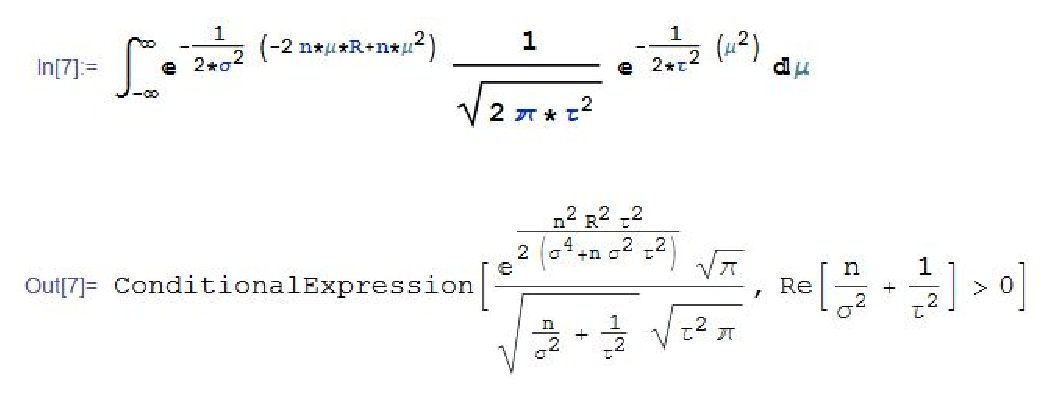
\includegraphics[width=6in]{integrate_out_mu2.eps}
%\end{center}
%\end{figure}
%\FloatBarrier

%And this result does not appear to be equal to $\normnot{0}{\overn{\sigsq} + \sigsq_\mu}$. \\


%\beqn
%\cprob{\Rlonetonl}{\sigsq} = h(\Rlonetonl ~|~ \sigsq) \oneoversqrt{\sigsq_\mu \parens{\frac{n_\ell}{\sigsq} + 1}} \exp{\frac{n_\ell^2 \Rbar_\ell^2 \sigsq_\mu}{2\parens{\sigma^4 + n_\ell\sigsq \sigsq_\mu}}}
%\eeqn

So now we substitue the above result into equation 1:

\begin{changemargin}{-0.5in}{0in}
\beqn
&& \frac{\cprob{\R}{T^*, \sigsq}}{\cprob{\R}{T, \sigsq}} \\
&=& \frac{h_L ~ \oneoversqrt{2\pi \parens{\frac{\sigsq}{n_{\ell_L}} + \sigsq_\mu}} ~\exp{-\oneover{2 \parens{\frac{\sigsq}{n_{\ell_L}} + \sigsq_\mu}} \Rbar_{\ell_L}^2} h_R ~ \oneoversqrt{2\pi \parens{\frac{\sigsq}{n_{\ell_R}} + \sigsq_\mu}} ~\exp{-\oneover{2 \parens{\frac{\sigsq}{n_{\ell_R}} + \sigsq_\mu}} \Rbar_{\ell_R}^2}}{h ~ \oneoversqrt{2\pi \parens{\frac{\sigsq}{n_\ell} + \sigsq_\mu}} ~\exp{-\oneover{2 \parens{\frac{\sigsq}{n_\ell} + \sigsq_\mu}} \Rbar_\ell^2}} \\
&=& \frac{h_L h_R}{h}  \sqrt{\frac{\cancel{2\pi} \parens{\frac{\sigsq}{n_\ell} + \sigsq_\mu}}{\cancel{2\pi} \parens{\frac{\sigsq}{n_{\ell_L}} + \sigsq_\mu} 2\pi \parens{\frac{\sigsq}{n_{\ell_R}} + \sigsq_\mu}}} \frac{~\exp{-\oneover{2 \parens{\frac{\sigsq}{n_{\ell_L}} + \sigsq_\mu}} \Rbar_{\ell_L}^2}  ~\exp{-\oneover{2 \parens{\frac{\sigsq}{n_{\ell_R}} + \sigsq_\mu}} \Rbar_{\ell_R}^2}}{\exp{-\oneover{2 \parens{\frac{\sigsq}{n_\ell} + \sigsq_\mu}} \Rbar_\ell^2}} \\
&=& \frac{h_L h_R}{h}  \sqrt{\frac{ \parens{\frac{\sigsq}{n_\ell} + \sigsq_\mu}}{ \parens{\frac{\sigsq}{n_{\ell_L}} + \sigsq_\mu} 2\pi \parens{\frac{\sigsq}{n_{\ell_R}} + \sigsq_\mu}}} \exp{\oneover{2 \parens{\frac{\sigsq}{n_\ell} + \sigsq_\mu}} \Rbar_\ell^2 -\oneover{2 \parens{\frac{\sigsq}{n_{\ell_L}} + \sigsq_\mu}} \Rbar_{\ell_L}^2 -\oneover{2 \parens{\frac{\sigsq}{n_{\ell_R}} + \sigsq_\mu}} \Rbar_{\ell_R}^2} \\
\eeqn
\end{changemargin}

%\beqn
%\frac{\cprob{\R}{T^*, \sigsq}}{\cprob{\R}{T, \sigsq}} &=& h\parens{\RLlonetonlL ~|~ \sigsq} \oneoversqrt{\sigsq_\mu \parens{\frac{n_{\ell_L}}{\sigsq} + 1}} ~~\exp{\frac{n_{\ell_L}^2 \Rbar_{\ell_L}^2 \sigsq_\mu}{2\parens{\sigma^4 + n_{\ell_L}\sigsq \sigsq_\mu}}} \\
%&& ~~\times h\parens{\RRlonetonlR ~|~ \sigsq} \oneoversqrt{\sigsq_\mu \parens{\frac{n_{\ell_R}}{\sigsq} + 1}} ~~\exp{\frac{n_{\ell_R}^2 \Rbar_{\ell_R}^2 \sigsq_\mu}{2\parens{\sigma^4 + n_{\ell_R}\sigsq \sigsq_\mu}}} \\
%&& ~~\times \inverse{h\parens{\Rlonetonl ~|~ \sigsq} \oneoversqrt{\sigsq_\mu \parens{\frac{n_\ell}{\sigsq} + 1}} ~~\exp{\dfrac{n_\ell^2 \Rbar_\ell^2 \sigsq_\mu}{2\parens{\sigma^4 + n_\ell\sigsq \sigsq_\mu}}}} \\
%\eeqn

Let's examine the ratio of the $h$ functions:

\begin{changemargin}{-1in}{0in}
\beqn
&& \frac{h_L h_R}{h} = \frac{\doneoversqrt{n_{\ell_L}} \doneover{\tothepow{2\pi\sigsq}{\overtwo{n_{\ell_L} - 1}}} ~\exp{-\oneover{2\sigsq} \sum_{i=1}^{n_{\ell_L}} \squared{R_{\ell_L, i} - \Rbar_{\ell_L}}} \doneoversqrt{n_{\ell_R}} \doneover{\tothepow{2\pi\sigsq}{\overtwo{n_{\ell_R} - 1}}} ~\exp{-\oneover{2\sigsq} \sum_{i=1}^{n_{\ell_R}} \squared{R_{\ell_R, i} - \Rbar_{\ell,R}}}}{\doneoversqrt{n_\ell} \doneover{\tothepow{2\pi\sigsq}{\overtwo{n_\ell - 1}}} ~\exp{-\oneover{2\sigsq} \sum_{i=1}^{n_\ell} \squared{R_{\ell_i} - \Rbar_\ell}}} \\
\eeqn
\end{changemargin}

Now note that:

\beqn
\frac{\doneover{\tothepow{2\pi\sigsq}{\overtwo{n_{\ell_L} - 1}}} \doneover{\tothepow{2\pi\sigsq}{\overtwo{n_{\ell_R} - 1}}}}{\doneover{\tothepow{2\pi\sigsq}{\overtwo{n_\ell - 1}}}} = \frac{\tothepow{2\pi\sigsq}{\overtwo{n_\ell - 1}}}{\tothepow{2\pi\sigsq}{\overtwo{n_\ell - 2}}} = \sqrt{2\pi\sigsq}
\eeqn

Grouping the rest of the terms inside and outside of the exponentiation:

\beqn
\frac{h_L h_R}{h} &=& \sqrt{\frac{2\pi\sigsq n_\ell}{n_{\ell_L}n_{\ell_R}}} ~\exp{-\oneover{2\sigsq}\parens{\underbrace{\sum_{i=1}^{n_{\ell_L}} \squared{R_{\ell_L, i} - \Rbar_{\ell_L}} + \sum_{i=1}^{n_{\ell_R}} \squared{R_{\ell_R, i} - \Rbar_{\ell,R}} - \sum_{i=1}^{n_\ell} \squared{R_{\ell_i} - \Rbar_\ell}}}}
\eeqn

Now let's take a look at the underbraced quantity:

\beqn
&=& \sum_{i=1}^{n_{\ell_L}} R_{\ell_L, i}^2 - 2n_{\ell_L}\Rbar_{\ell_L}^2 + n_{\ell_L}\Rbar_{\ell_L}^2 +\sum_{i=1}^{n_{\ell_R}} R_{\ell_R, i}^2 - 2n_{\ell_R}\Rbar_{\ell_R}^2 + n_{\ell_R}\Rbar_{\ell_R}^2 - \sum_{i=1}^{n_{\ell}} R_{\ell, i}^2 + 2n_{\ell}\Rbar_{\ell}^2 - n_{\ell}\Rbar_{\ell}^2 \\
&=& \cancel{\sum_{i=1}^{n_{\ell_L}} R_{\ell_L, i}^2} - 2n_{\ell_L}\Rbar_{\ell_L}^2 + n_{\ell_L}\Rbar_{\ell_L}^2 + \cancel{\sum_{i=1}^{n_{\ell_R}} R_{\ell_R, i}^2} - 2n_{\ell_R}\Rbar_{\ell_R}^2 + n_{\ell_R}\Rbar_{\ell_R}^2 - \cancel{\sum_{i=1}^{n_{\ell}} R_{\ell, i}^2} + 2n_{\ell}\Rbar_{\ell}^2 - n_{\ell}\Rbar_{\ell}^2 \\
&=& n_{\ell}\Rbar_{\ell}^2 - n_{\ell_L}\Rbar_{\ell_L}^2 - n_{\ell_R}\Rbar_{\ell_R}^2
\eeqn

Thus, we can arrive at the $h$ ratio's final expression:

\beqn
\frac{h_L h_R}{h} &=& \sqrt{\frac{2\pi\sigsq n_\ell}{n_{\ell_L}n_{\ell_R}}} ~\exp{-\oneover{2\sigsq} \parens{n_{\ell}\Rbar_{\ell}^2 - n_{\ell_L}\Rbar_{\ell_L}^2 - n_{\ell_R}\Rbar_{\ell_R}^2}} \\
\eeqn

Now, putting it all together:

\begin{changemargin}{-0.5in}{0in}
\beqn
&& \frac{\cprob{\R}{T^*, \sigsq}}{\cprob{\R}{T, \sigsq}} \\
&=& \sqrt{\frac{\cancel{2\pi} \sigsq n_\ell}{n_{\ell_L}n_{\ell_R}}} \sqrt{\frac{ \parens{\frac{\sigsq}{n_\ell} + \sigsq_\mu}}{ \parens{\frac{\sigsq}{n_{\ell_L}} + \sigsq_\mu} \cancel{2\pi} \parens{\frac{\sigsq}{n_{\ell_R}} + \sigsq_\mu}}} ~\exp{-\oneover{2\sigsq} \parens{n_{\ell}\Rbar_{\ell}^2 - n_{\ell_L}\Rbar_{\ell_L}^2 - n_{\ell_R}\Rbar_{\ell_R}^2}} \times \\
&& \exp{\half \parens{\oneover{\parens{\frac{\sigsq}{n_\ell} + \sigsq_\mu}} \Rbar_\ell^2 -\oneover{ \parens{\frac{\sigsq}{n_{\ell_L}} + \sigsq_\mu}} \Rbar_{\ell_L}^2 -\oneover{\parens{\frac{\sigsq}{n_{\ell_R}} + \sigsq_\mu}} \Rbar_{\ell_R}^2}} \\
&=& \sqrt{\frac{\sigsq n_\ell}{n_{\ell_L}n_{\ell_R}} \frac{ \parens{\frac{\sigsq}{n_\ell} + \sigsq_\mu}}{ \parens{\frac{\sigsq}{n_{\ell_L}} + \sigsq_\mu} \parens{\frac{\sigsq}{n_{\ell_R}} + \sigsq_\mu}}} ~\exp{\oneover{2\sigsq} \parens{n_{\ell_L}\Rbar_{\ell_L}^2 + n_{\ell_R}\Rbar_{\ell_R}^2 - n_{\ell}\Rbar_{\ell}^2}} \times \\
&&  \exp{\oneover{2\sigsq} \parens{\oneover{\parens{\frac{1}{n_\ell} + \frac{\sigsqmu}{\sigsq}}} \Rbar_\ell^2 -\oneover{\parens{\frac{1}{n_{\ell_L}} + \frac{\sigsqmu}{\sigsq}}} \Rbar_{\ell_L}^2 -\oneover{\parens{\frac{1}{n_{\ell_R}} + \frac{\sigsqmu}{\sigsq}}} \Rbar_{\ell_R}^2}} \\
&=& \underbrace{\sqrt{\frac{\sigsq \parens{\sigsq + \sigsq_\mu n_{\ell_L}}}{ \parens{\sigsq + \sigsq_\mu n_{\ell_L}} \parens{\sigsq + \sigsq_\mu n_{\ell_R}}}}}_c \times \\
&&  \exp{\oneover{2\sigsq} \parens{\parens{\oneover{\parens{\frac{1}{n_\ell} + \frac{\sigsqmu}{\sigsq}}} - n_\ell} \Rbar_\ell^2 -\parens{\oneover{\parens{\frac{1}{n_{\ell_L}} + \frac{\sigsqmu}{\sigsq}}} + n_{\ell_L}} \Rbar_{\ell_L}^2 - \parens{\oneover{\parens{\frac{1}{n_{\ell_R}} + \frac{\sigsqmu}{\sigsq}}} + n_{\ell_R}} \Rbar_{\ell_R}^2}} \\
&=& c ~\exp{\oneover{2\sigsq} \parens{-\parens{\frac{\frac{\sigsqmu n_{\ell}}{\sigsq}}{\parens{\frac{1}{n_\ell} + \frac{\sigsqmu}{\sigsq}}}} \Rbar_\ell^2 + \parens{\frac{\frac{\sigsqmu n_{\ell_L}}{\sigsq}}{\parens{\frac{1}{n_{\ell_L}} + \frac{\sigsqmu}{\sigsq}}}} \Rbar_{\ell_L}^2 + \parens{\frac{\frac{\sigsqmu n_{\ell_R}}{\sigsq}}{\parens{\frac{1}{n_{\ell_R}} + \frac{\sigsqmu}{\sigsq}}}} \Rbar_{\ell_R}^2}} \\
&=& c ~\exp{\oneover{2\sigsq} \parens{\parens{\frac{\sigsqmu n_{\ell_L}}{\parens{\frac{\sigsq}{n_{\ell_L}} + \sigsqmu}}} \Rbar_{\ell_L}^2 + \parens{\frac{\sigsqmu n_{\ell_R}}{\parens{\frac{\sigsq}{n_{\ell_R}} + \sigsqmu}}} \Rbar_{\ell_R}^2} - \parens{\frac{\sigsqmu n_{\ell}}{\parens{\frac{\sigsq}{n_\ell} + \sigsqmu}}} \Rbar_\ell^2} \\
&=& \sqrt{\frac{\sigsq \parens{\sigsq + \sigsq_\mu n_{\ell_L}}}{ \parens{\sigsq + \sigsq_\mu n_{\ell_L}} \parens{\sigsq + \sigsq_\mu n_{\ell_R}}}} \exp{\frac{\sigsqmu}{2\sigsq} \parens{ \frac{\squared{\sum_{i=1}^{n_{\ell_L}} R_{\ell_L, i}}}{\parens{\sigsq + n_{\ell_L}\sigsqmu}} + \frac{\squared{\sum_{i=1}^{n_{\ell_R}} R_{\ell_R, i}}}{\parens{\sigsq + n_{\ell_R}\sigsqmu}} - \frac{\squared{\sum_{i=1}^{n_{\ell}} R_{\ell, i}}}{\parens{\sigsq + n_\ell \sigsqmu}}}} \\
\eeqn
\end{changemargin}


\subsubsection*{Strategy \#2 --- Integral Computation in Mathematica}

Let's factorize the $\iid$ normal likelihood like the following:

\beqn
\prob{\Rlonetonl | \mu, \sigsq} &=& \oneover{\tothepow{2\pi\sigsq}{n_\ell / 2}} ~\exp{-\oneover{2\sigsq} \sum_{i=1}^{n_\ell} \squared{R_{\ell_i} - \mu}} \\
&=& \oneover{\tothepow{2\pi\sigsq}{n_\ell / 2}} ~\exp{-\oneover{2\sigsq} \sum_{i=1}^{n_\ell} R_{\ell_i}^2} \underbrace{\exp{-\oneover{2\sigsq} \parens{-2n_\ell \mu \Rbar_\ell + n_\ell \musq}}}_g \\
%&=& h(\Rlonetonl ~|~ \sigsq) \cdot g(\Rbar_\ell ~|~ \mu, \sigsq) \\
\eeqn

Now, let's try to build the ratio:

\small
\begin{changemargin}{-1in}{0in}
\beqn
&& \frac{\cprob{\R}{T^*, \sigsq}}{\cprob{\R}{T, \sigsq}} \\
&=& \frac{\cprob{\RLlonetonlL}{\sigsq} \cprob{\RRlonetonlR}{\sigsq}}{\cprob{\Rlonetonl}{\sigsq}} \\
&=& \frac{\myint{\mu}{\reals}{}{\cprob{\RLlonetonlL}{\mu, \sigsq}\prob{\mu}} ~~ \myint{\mu}{\reals}{}{\cprob{\RRlonetonlR}{\mu, \sigsq}\prob{\mu}}}{\myint{\mu}{\reals}{}{\cprob{\Rlonetonl}{\mu, \sigsq}\prob{\mu}}} \\
&=& \frac{\oneover{\tothepow{2\pi\sigsq}{n_{\ell_L} / 2}} ~\exp{-\oneover{2\sigsq} \sum_{i=1}^{n_{\ell_L}} R_{{\ell_L}_i}^2} \parens{\myint{\mu}{\reals}{}{g_{\ell_L} \prob{\mu}}}~ \oneover{\tothepow{2\pi\sigsq}{n_{\ell_R} / 2}}  ~\exp{-\oneover{2\sigsq} \sum_{i=1}^{n_{\ell_R}} R_{{\ell_R}_i}^2} \parens{\myint{\mu}{\reals}{}{g_{\ell_R} \prob{\mu}}}}{\oneover{\tothepow{2\pi\sigsq}{n_\ell / 2}} ~\exp{-\oneover{2\sigsq} \sum_{i=1}^{n_\ell} R_{\ell_i}^2} \parens{\myint{\mu}{\reals}{}{g_{\ell} \prob{\mu}}}} \\
&=& \frac{\cancel{\oneover{\tothepow{2\pi\sigsq}{n_{\ell_L} / 2}}} ~\cancel{\exp{-\oneover{2\sigsq} \sum_{i=1}^{n_{\ell_L}} R_{{\ell_L}_i}^2}} \parens{\myint{\mu}{\reals}{}{g_{\ell_L} \prob{\mu}}}~ \cancel{\oneover{\tothepow{2\pi\sigsq}{n_{\ell_R} / 2}}}  ~\cancel{\exp{-\oneover{2\sigsq}} \sum_{i=1}^{n_{\ell_R}} R_{{\ell_R}_i}^2} \parens{\myint{\mu}{\reals}{}{g_{\ell_R} \prob{\mu}}}}{\cancel{\oneover{\tothepow{2\pi\sigsq}{n_\ell / 2}}} ~\cancel{\exp{-\oneover{2\sigsq} \sum_{i=1}^{n_\ell} R_{\ell_i}^2}} \parens{\myint{\mu}{\reals}{}{g_{\ell} \prob{\mu}}}} \\
&=& \frac{\myint{\mu}{\reals}{}{g_{\ell_L} \prob{\mu}} \myint{\mu}{\reals}{}{g_{\ell_R} \prob{\mu}}}{\myint{\mu}{\reals}{}{g_{\ell} \prob{\mu}}} \\
&=& \frac{\myint{\mu}{\reals}{}{g_{\ell_L} \cancel{\oneoversqrt{2\pi\sigsqmu}} \exp{-\oneover{2\sigsqmu} \musq}} \myint{\mu}{\reals}{}{g_{\ell_R} \oneoversqrt{2\pi\sigsq_\mu} \exp{-\oneover{2\sigsqmu} \musq}}}{\myint{\mu}{\reals}{}{g_{\ell} \cancel{\oneoversqrt{2\pi\sigsq_\mu}} \exp{-\oneover{2\sigsqmu} \musq}}} \\
&=& \oneoversqrt{2\pi\sigsq_\mu} \frac{\myint{\mu}{\reals}{}{\exp{-\oneover{2\sigsq} \parens{-2n_{\ell_L} \mu \Rbar_{\ell_L} + n_{\ell_L} \musq}} \exp{-\oneover{2\sigsqmu} \musq}} \myint{\mu}{\reals}{}{\exp{-\oneover{2\sigsq} \parens{-2n_{\ell_L} \mu \Rbar_{\ell_L} + n_{\ell_L} \musq}}  \exp{-\oneover{2\sigsqmu} \musq}}}{\underbrace{\myint{\mu}{\reals}{}{\exp{-\oneover{2\sigsq} \parens{-2n_\ell \mu \Rbar_\ell + n_\ell \musq}} \exp{-\oneover{2\sigsqmu} \musq}}}} \\
\eeqn
\end{changemargin}
\normalsize

Let's evaluate the underbraced integral using Mathematica:

%The problem here is that $g$ is not a likelihood. So I don't know how to do that margining trick with $\normnot{0}{\overn{\sigsq}} \star \normnot{0}{\sigsq_\mu} = \normnot{0}{\overn{\sigsq} + \sigsq_\mu}$. So I think I have to do the integral manually using Mathematica:

\beqn
\int_\reals g(\Rbar_\ell ~|~ \mu, \sigsq) \prob{\mu; \sigsq_\mu} d\mu &=& \int_\reals \exp{-\oneover{2\sigsq} \parens{-2n_\ell \mu \Rbar_\ell + n_\ell \musq}} \exp{-\oneover{2\sigsq_\mu} \musq} d\mu \\
&=& \sqrt{\frac{2\pi}{\frac{n_\ell}{\sigsq} + \oneover{\sigsqmu}}} \exp{\frac{n_\ell^2 \Rbar_\ell^2 \sigsq_\mu}{2\sigsq\parens{\sigsq + n_\ell \sigsq_\mu}}} \\
%\Rightarrow \cprob{\Rlonetonl}{\sigsq} &\propto& \oneoversqrt{\sigsq_\mu \parens{\frac{n_\ell}{\sigsq} + 1}} \exp{\frac{n_\ell^2 \Rbar_\ell^2 \sigsq_\mu}{2\sigsq\parens{\sigsq + n_\ell \sigsq_\mu}}} \\
\eeqn

So now we have:

\small
\begin{changemargin}{-1in}{0in}
\beqn
&& \frac{\cprob{\R}{T^*, \sigsq}}{\cprob{\R}{T, \sigsq}} \\
&=& \oneoversqrt{\cancel{2\pi}\sigsq_\mu} \frac{\sqrt{\dfrac{\cancel{2\pi}}{\frac{n_{\ell_L}}{\sigsq} + \oneover{\sigsqmu}}} \exp{\dfrac{n_{\ell_L}^2 \Rbar_{\ell_L}^2 \sigsq_\mu}{2\sigsq\parens{\sigsq + n_{\ell_L} \sigsq_\mu}}} \sqrt{\dfrac{\cancel{2\pi}}{\frac{n_{\ell_R}}{\sigsq} + \oneover{\sigsqmu}}} \exp{\dfrac{n_{\ell_R}^2 \Rbar_{\ell_R}^2 \sigsq_\mu}{2\sigsq\parens{\sigsq + n_{\ell_R} \sigsq_\mu}}}}{\sqrt{\dfrac{\cancel{2\pi}}{\frac{n_\ell}{\sigsq} + \oneover{\sigsqmu}}} \exp{\dfrac{n_\ell^2 \Rbar_\ell^2 \sigsq_\mu}{2\sigsq\parens{\sigsq + n_\ell \sigsq_\mu}}}} \\
&=& \sqrt{\frac{\frac{n_\ell}{\sigsq} + \oneover{\sigsqmu}}{\sigsqmu \parens{\frac{n_{\ell_L}}{\sigsq} + \oneover{\sigsqmu}}\parens{\frac{n_{\ell_R}}{\sigsq} + \oneover{\sigsqmu}}}} ~~\exp{\frac{\sigsq_\mu}{2\sigsq} \parens{\frac{n_{\ell_L}^2 \Rbar_{\ell_L}^2}{\sigsq + n_{\ell_L}\sigsq_\mu} + \frac{n_{\ell_R}^2 \Rbar_{\ell_R}^2}{\sigsq + n_{\ell_R}\sigsq_\mu} - \frac{n_\ell^2 \Rbar_\ell^2}{\sigsq + n_\ell \sigsq_\mu}}} \\
&=& \sqrt{\frac{\sigsq \parens{\sigsq + n_\ell \sigsqmu}}{\parens{\sigsq + n_{\ell_L} \sigsqmu}\parens{\sigsq + n_{\ell_R} \sigsqmu}}}~~\exp{\frac{\sigsq_\mu}{2\sigsq} \parens{\frac{\squared{\sum_{i=1}^{n_{\ell_L}} R_{\ell_L, i}}}{\sigsq + n_{\ell_L}\sigsq_\mu} + \frac{\squared{\sum_{i=1}^{n_{\ell_R}} R_{\ell_R, i}}}{\sigsq + n_{\ell_R}\sigsq_\mu} - \frac{\squared{\sum_{i=1}^{n_{\ell}} R_{\ell, i}}}{\sigsq + n_\ell \sigsq_\mu}}} \\
\eeqn
\end{changemargin}
\normalsize

%\begin{figure}
%\begin{center}
%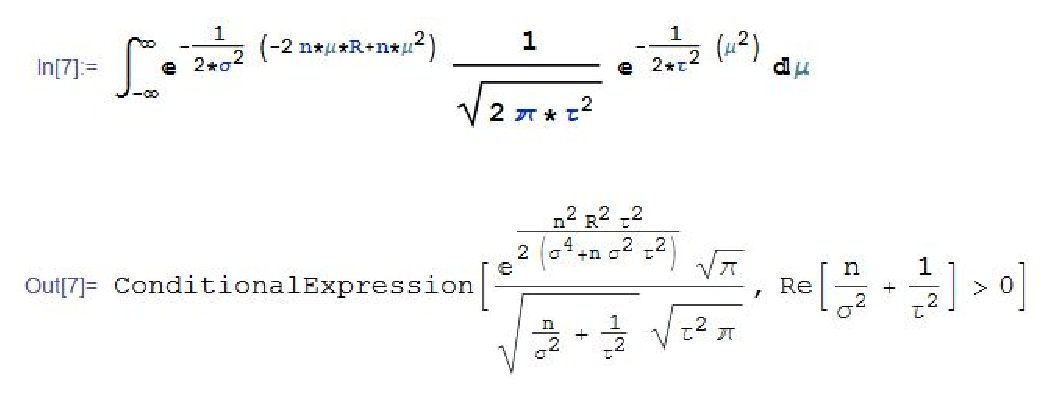
\includegraphics[width=6in]{integrate_out_mu2.eps}
%\end{center}
%\end{figure}
%\FloatBarrier


%\beqn
%&& \frac{h\parens{\RLlonetonlL ~|~ \sigsq}h\parens{\RRlonetonlR ~|~ \sigsq}}{h\parens{\Rlonetonl ~|~ \sigsq}} \\
%&=& \frac{\doneover{\tothepow{2\pi\sigsq}{n_{\ell_L} / 2}} ~\exp{-\doneover{2\sigsq} \sum_{i=1}^{n_{\ell_L}} R_{\ell_i}^2} \doneover{\tothepow{2\pi\sigsq}{n_{\ell_R} / 2}} ~\exp{-\doneover{2\sigsq} \sum_{i=1}^{n_{\ell_R}} R_{\ell_i}^2}}{\doneover{\tothepow{2\pi\sigsq}{n_\ell / 2}} ~\exp{-\doneover{2\sigsq} \sum_{i=1}^{n_\ell} R_{\ell_i}^2}} \\
%&=& \frac{\doneover{\tothepow{2\pi\sigsq}{n_\ell / 2}} ~\exp{-\doneover{2\sigsq} \sum_{i=1}^{n_\ell} R_{\ell_i}^2}}{\doneover{\tothepow{2\pi\sigsq}{n_\ell / 2}} ~\exp{-\doneover{2\sigsq} \sum_{i=1}^{n_\ell} R_{\ell_i}^2}} = 1 \eqncomment{since $n_\ell = n_{\ell_R} + n_{\ell_L}$}
%\eeqn


%\begin{changemargin}{-0.5in}{0in}
%\beqn
%\frac{\cprob{\R}{T^*, \sigsq}}{\cprob{\R}{T, \sigsq}} &=& \frac{\oneoversqrt{\sigsq_\mu \parens{\frac{n_{\ell_L}}{\sigsq} + 1}} \oneoversqrt{\sigsq_\mu \parens{\frac{n_{\ell_R}}{\sigsq} + 1}} ~~\exp{\dfrac{n_{\ell_L}^2 \Rbar_{\ell_L}^2 \sigsq_\mu}{2\parens{\sigma^4 + n_{\ell_L}\sigsq \sigsq_\mu}}} ~~\exp{\dfrac{n_{\ell_R}^2 \Rbar_{\ell_R}^2 \sigsq_\mu}{2\parens{\sigma^4 + n_{\ell_R}\sigsq \sigsq_\mu}}}}{\oneoversqrt{\sigsq_\mu \parens{\frac{n_\ell}{\sigsq} + 1}} ~~\exp{\dfrac{n_\ell^2 \Rbar_\ell^2 \sigsq_\mu}{2\parens{\sigma^4 + n_\ell\sigsq \sigsq_\mu}}}} \\
%&=& \sqrt{\frac{\sigsq \parens{n_\ell + \sigsq}}{\sigsq_\mu \parens{n_{\ell_L} + \sigsq}\parens{n_{\ell_R} + \sigsq}}} ~~\exp{\frac{\sigsq_\mu}{2\sigsq} \parens{\frac{\overbrace{n_{\ell_L}^2 \Rbar_{\ell_L}^2}}{\sigsq + n_{\ell_L}\sigsq_\mu} + \frac{\overbrace{n_{\ell_R}^2 \Rbar_{\ell_R}^2}}{\sigsq + n_{\ell_R}\sigsq_\mu} - \frac{\overbrace{n_\ell^2 \Rbar_\ell^2}}{\sigsq + n_\ell \sigsq_\mu}}} \\
%\eeqn
%\end{changemargin}

%Note how the ratio is only a function of the $\sum R_i$'s which makes calculations efficient.

%Let's think about what's really driving this ratio. Consider $\sigsq = \sigsqmu = 1$ and $n_\ell = 10$ with an equal split in left and right daughter leaves. That would mean that the ratio would be:
%
%\beqn
%\sqrt{\frac{11}{36}}~~\exp{\half \parens{\frac{\squared{\sum_{i=1}^{n_{\ell_L}} R_{\ell_L, i}}}{6} + \frac{\squared{\sum_{i=1}^{n_{\ell_L}} R_{\ell_R, i}}}{6} - \frac{\squared{\sum_{i=1}^{n_{\ell_L}} R_{\ell, i}}}{11}}} \\
%\eeqn



\subsubsection*{Strategy \#3 --- Completing the Square}

Recall that:

\begin{changemargin}{-0.5in}{0in}
\beqn
\prob{\Rlonetonl | \mu, \sigsq} &=& \oneover{\tothepow{2\pi\sigsq}{n_\ell / 2}} ~\exp{-\oneover{2\sigsq} \sum_{i=1}^{n_\ell} \squared{R_{\ell_i} - \mu}} \\
&=& \oneover{\tothepow{2\pi\sigsq}{n_\ell / 2}} ~\exp{-\oneover{2\sigsq} \parens{n_\ell \squared{\Rbar_\ell - \mu} + \sum_{i=1}^{n_\ell} \squared{R_{\ell_i} - \Rbar_\ell}}} \\
&=& \oneover{\tothepow{2\pi\sigsq}{n_\ell / 2}} ~\exp{-\oneover{2\sigsq} \sum_{i=1}^{n_\ell} \squared{R_{\ell_i} - \Rbar_\ell}} ~\exp{-\frac{n_\ell}{2\sigsq} \squared{\Rbar_\ell - \mu}} \\
&=& \oneover{\tothepow{2\pi\sigsq}{n_\ell / 2}} ~\exp{-\oneover{2\sigsq} \sum_{i=1}^{n_\ell} \squared{R_{\ell_i} - \Rbar_\ell}} ~\exp{-\frac{n_\ell}{2\sigsq} \parens{\Rbar_\ell^2 - 2\Rbar_\ell \mu + \musq}} \\
\eeqn
\end{changemargin}

which means that:

\beqn
\cprob{\Rlonetonl}{\sigsq} &=& \oneover{\tothepow{2\pi\sigsq}{n_\ell / 2}} ~\exp{-\oneover{2\sigsq} \sum_{i=1}^{n_\ell} \squared{R_{\ell_i} - \Rbar_\ell}} \times \\
&& \myint{\mu}{\reals}{}{\exp{-\frac{n_\ell}{2\sigsq} \parens{\Rbar_\ell^2 - 2\Rbar_\ell \mu + \musq}}\oneoversqrt{2\pi\sigsq_\mu}\exp{-\oneover{2\sigsqmu} \musq}} \\
&=& \oneover{\tothepow{2\pi\sigsq}{n_\ell / 2}} ~\exp{-\oneover{2\sigsq} \sum_{i=1}^{n_\ell} \squared{R_{\ell_i} - \Rbar_\ell}} \times \\
&& \oneoversqrt{2\pi\sigsq_\mu} \myint{\mu}{\reals}{}{\exp{-\frac{n_\ell}{2\sigsq} \parens{\Rbar_\ell^2 - 2\Rbar_\ell \mu + \musq} -\oneover{2\sigsqmu} \musq}} \\
&=& \oneover{\tothepow{2\pi\sigsq}{n_\ell / 2}} ~\exp{-\oneover{2\sigsq} \sum_{i=1}^{n_\ell} \squared{R_{\ell_i} - \Rbar_\ell}} \times \\
&& \oneoversqrt{2\pi\sigsq_\mu} \myint{\mu}{\reals}{}{\exp{\underbrace{\parens{-\frac{n_\ell}{2\sigsq} - \oneover{2\sigsqmu}}\musq + \parens{\frac{\Rbar_\ell n_\ell}{\sigsq}} \mu} - \frac{n_\ell \Rbar_\ell^2}{2\sigsq}}} \\
\eeqn

Now let's complete the square of the underbraced above. We want it to look like $c\squared{d-\mu} = c\musq - 2cd\mu + cd^2$. Already we have $c$, the factor multiplying $\musq$, so then $d$ becomes (using the $\mu$ term above):

\beqn
d = \frac{\Rbar_\ell n_\ell}{-2c\sigsq} = \frac{\Rbar_\ell n_\ell}{-2 \parens{-\frac{n_\ell}{2\sigsq} - \oneover{2\sigsqmu}} \sigsq} = \frac{\Rbar_\ell n_\ell}{n_\ell + \frac{\sigsq}{\sigsqmu}}
\eeqn

and the final $cd^2$ term becomes:

\beqn
cd^2 = c \squaredfrac{\Rbar_\ell n_\ell}{-2c\sigsq} = \frac{\Rbar_\ell^2 n_\ell^2}{4c \sigma^4} =  \frac{\Rbar_\ell^2 n_\ell^2}{4\parens{-\frac{n_\ell}{2\sigsq} - \oneover{2\sigsqmu}} \sigma^4} = \frac{\Rbar_\ell^2 n_\ell^2}{-2\parens{\frac{n_\ell}{\sigsq} + \oneover{\sigsqmu}} \sigma^4} = \frac{\Rbar_\ell^2 n_\ell^2}{-2\sigsq\parens{n_\ell + \frac{\sigsq}{\sigsqmu}}}
\eeqn

Returning to our margined expression, we subtract and add the $cd^2$ term inside the exponentiation:

\small
\begin{changemargin}{-0.5in}{0in}
\beqn
\cprob{\Rlonetonl}{\sigsq} &=& \oneover{\tothepow{2\pi\sigsq}{n_\ell / 2}} ~\exp{-\oneover{2\sigsq} \sum_{i=1}^{n_\ell} \squared{R_{\ell_i} - \Rbar_\ell}} \oneoversqrt{2\pi\sigsq_\mu}\times \\
&&  \myint{\mu}{\reals}{}{\exp{\underbrace{\parens{-\frac{n_\ell}{2\sigsq} - \oneover{2\sigsqmu}}\musq + \parens{\frac{\Rbar_\ell}{\sigsq}} \mu - \frac{\Rbar_\ell^2 n_\ell^2}{2\sigsq\parens{n_\ell + \frac{\sigsq}{\sigsqmu}}}} + \frac{\Rbar_\ell^2 n_\ell^2}{2\sigsq\parens{n_\ell + \frac{\sigsq}{\sigsqmu}}} - \frac{n_\ell \Rbar_\ell^2}{2\sigsq}} } \\
\eeqn
\end{changemargin}
\normalsize

So the underbraced is the ``square'' and we pull the last two terms out (because they are not functions of $\mu$) to arrive at:

\begin{changemargin}{-0.5in}{0in}
\beqn
\cprob{\Rlonetonl}{\sigsq} &=& \oneover{\tothepow{2\pi\sigsq}{n_\ell / 2}} ~\exp{-\oneover{2\sigsq} \sum_{i=1}^{n_\ell} \squared{R_{\ell_i} - \Rbar_\ell}} \oneoversqrt{2\pi\sigsq_\mu} \times \\
&& ~\exp{\frac{\Rbar_\ell^2 n_\ell^2}{2\sigsq\parens{n_\ell + \frac{\sigsq}{\sigsqmu}}}- \frac{n_\ell \Rbar_\ell^2}{2\sigsq}} \myint{\mu}{\reals}{}{\exp{\parens{\underbrace{-\frac{n_\ell}{2\sigsq} - \oneover{2\sigsqmu}}}\squared{\mu - \frac{\Rbar_\ell}{n_\ell + \frac{\sigsq}{\sigsqmu}}}}} \\
\eeqn
\end{changemargin}

Note how the integral is now the Gaussian integral with the $-\oneover{2\sigsq_*}$ parameter underbraced. Hence it will integrate to $\sqrt{2\pi\sigsq_*}$ and the expression becomes:

\begin{changemargin}{-0.5in}{0in}
\beqn
\cprob{\Rlonetonl}{\sigsq} &=& \oneover{\tothepow{2\pi\sigsq}{n_\ell / 2}} ~\exp{-\oneover{2\sigsq} \sum_{i=1}^{n_\ell} \squared{R_{\ell_i} - \Rbar_\ell}} \times \\
&& \oneoversqrt{2\pi\sigsq_\mu} ~\exp{\frac{\Rbar_\ell^2 n_\ell^2}{2\sigsq\parens{n_\ell + \frac{\sigsq}{\sigsqmu}}}- \frac{n_\ell \Rbar_\ell^2}{2\sigsq}} \sqrt{2\pi \oneover{\frac{n_\ell}{\sigsq} + \oneover{\sigsqmu}}} \\
&=& \oneover{\tothepow{2\pi\sigsq}{n_\ell / 2}} \sqrt{ \frac{\sigsq}{\sigsq + n_\ell \sigsqmu}}  \times \\
&& \exp{-\oneover{2\sigsq} \sum_{i=1}^{n_\ell} \squared{R_{\ell_i} - \Rbar_\ell}} \exp{\frac{\Rbar_\ell^2 n_\ell^2}{2\sigsq\parens{n_\ell + \frac{\sigsq}{\sigsqmu}}}- \frac{n_\ell \Rbar_\ell^2}{2\sigsq}} \\
\eeqn
\end{changemargin}

So now we're ready to calculate the likelihood ratio.

\begin{changemargin}{-0.75in}{0in}
\beqn
&& \frac{\cprob{\R}{T^*, \sigsq}}{\cprob{\R}{T, \sigsq}} \\
&=& \frac{\cprob{\RLlonetonlL}{\sigsq} \cprob{\RRlonetonlR}{\sigsq}}{\cprob{\Rlonetonl}{\sigsq}} \\
&=& \frac{\cancel{\oneover{\tothepow{2\pi\sigsq}{n_{\ell_L} / 2}}} ~ \exp{\frac{\Rbar_{\ell_L}^2 n_\ell^2}{2\sigsq\parens{n_{\ell_L} + \frac{\sigsq}{\sigsqmu}}}- \frac{n_{\ell_L} \Rbar_{\ell_L}^2 }{2\sigsq}} \sqrt{ \frac{\cancel{\sigsq}}{\sigsq + n_{\ell_L} \sigsqmu}} \cancel{\oneover{\tothepow{2\pi\sigsq}{n_{\ell_R} / 2}}} ~ \exp{\frac{\Rbar_{\ell_R}^2 n_\ell^2}{2\sigsq\parens{n_{\ell_R} + \frac{\sigsq}{\sigsqmu}}}- \frac{n_{\ell_R} \Rbar_{\ell_R}^2}{2\sigsq}} \sqrt{ \frac{\sigsq}{\sigsq + n_{\ell_R} \sigsqmu}} }{\cancel{\oneover{\tothepow{2\pi\sigsq}{n_\ell / 2}}} ~ \exp{\frac{\Rbar_\ell^2 n_\ell^2}{2\sigsq\parens{n_\ell + \frac{\sigsq}{\sigsqmu}}}- \frac{n_\ell \Rbar_\ell^2}{2\sigsq}} \sqrt{ \frac{\cancel{\sigsq}}{\sigsq + n_\ell \sigsqmu}}} \times \\
&& \exp{\underbrace{-\oneover{2\sigsq}\parens{\sum_{i=1}^{n_{\ell_L}} \squared{R_{\ell_L, i} - \Rbar_{\ell_L}} + \sum_{i=1}^{n_{\ell_R}} \squared{R_{\ell_R, i} - \Rbar_{\ell,R}} - \sum_{i=1}^{n_\ell} \squared{R_{\ell_i} - \Rbar_\ell}}}}
\eeqn
\end{changemargin}

We've calculate the underbraced before in the strategy \#1 section. We now substitute, factor, and collect terms:

\beqn
&=& \underbrace{\sqrt{\frac{\sigsq \parens{\sigsq + n_\ell \sigsqmu}}{\parens{\sigsq + n_{\ell_L} \sigsqmu}\parens{\sigsq + n_{\ell_R} \sigsqmu}}}}_c  \times \\ 
&& \exp{\oneover{2\sigsq} \parens{\frac{\Rbar_{\ell_L}^2 n_{\ell_L}^2}{\parens{n_{\ell_L} + \frac{\sigsq}{\sigsqmu}} }- n_{\ell_L}\Rbar_{\ell_L}^2 + \frac{\Rbar_{\ell_R}^2 n_{\ell_R}^2}{\parens{n_{\ell_R} + \frac{\sigsq}{\sigsqmu}}}- n_{\ell_R}\Rbar_{\ell_R}^2 - \frac{\Rbar_{\ell}^2 n_\ell^2}{\parens{n_{\ell} + \frac{\sigsq}{\sigsqmu}}} + n_\ell\Rbar_\ell^2}} \times \\
&& \exp{\oneover{2\sigsq} \parens{n_{\ell_L}\Rbar_{\ell_L}^2 + n_{\ell}\Rbar_{\ell}^2 - n_{\ell}\Rbar_{\ell}^2}} \\
&=& c~\exp{\frac{\sigsqmu}{2\sigsq} \parens{\parens{\frac{n_{\ell_L}^2}{\sigsqmu n_{\ell_L} +\sigsq}} \Rbar_{\ell_L}^2 + \parens{\frac{n_{\ell_R}^2}{\sigsqmu n_{\ell_R} + \sigsq}} \Rbar_{\ell_R}^2 - \parens{\frac{n_\ell^2}{\sigsqmu n_{\ell} + \sigsq}} \Rbar_{\ell}^2}} \\
&=& \sqrt{\frac{\sigsq \parens{\sigsq + n_\ell \sigsqmu}}{\parens{\sigsq + n_{\ell_L} \sigsqmu}\parens{\sigsq + n_{\ell_R} \sigsqmu}}}~~\exp{\frac{\sigsq_\mu}{2\sigsq} \parens{\frac{\squared{\sum_{i=1}^{n_{\ell_L}} R_{\ell_L, i}}}{\sigsq + n_{\ell_L}\sigsq_\mu} + \frac{\squared{\sum_{i=1}^{n_{\ell_R}} R_{\ell_R, i}}}{\sigsq + n_{\ell_R}\sigsq_\mu} - \frac{\squared{\sum_{i=1}^{n_{\ell}} R_{\ell, i}}}{\sigsq + n_\ell \sigsq_\mu}}} \\
\eeqn

We've now computed this using three different methods, so it must be correct?\\

In log form, this becomes:

\inblue{
\beqn
&& \half \parens{\natlog{\sigsq} +\natlog{\sigsq + n_\ell \sigsqmu} -\natlog{\sigsq + n_{\ell_L} \sigsqmu} - \natlog{\sigsq + n_{\ell_R} \sigsqmu}} + \\
&& \frac{\sigsq_\mu}{2\sigsq} \parens{\frac{\squared{\sum_{i=1}^{n_{\ell_L}} R_{\ell_L, i}}}{\sigsq + n_{\ell_L}\sigsq_\mu} + \frac{\squared{\sum_{i=1}^{n_{\ell_R}} R_{\ell_R, i}}}{\sigsq + n_{\ell_R}\sigsq_\mu} - \frac{\squared{\sum_{i=1}^{n_{\ell}} R_{\ell, i}}}{\sigsq + n_\ell \sigsq_\mu}}
\eeqn
}

\subsubsection*{Tree Structure Ratio}

Remember the prior form on trees: 

\beqn
\prob{T} &=& \prod_{\eta \in \Hleaves} \parens{1 - \probsplit{\eta}}  \prod_{\eta \in \Hint} \probsplit{\eta} \prod_{\eta \in \Hint} \probrule{\eta} \\
\eeqn

Remember from CGM98 that the probability of splitting on a given node $\eta$ is driven by two hyperparameters, $\alpha$ and $\beta$ in the following way where $d_\eta$ is the depth of the $\eta$ node:

\beqn
\probsplit{\eta} = \frac{\alpha}{\tothepow{1 + d_\eta}{\beta}}
\eeqn

The probability of assigning the specific rule, $\prob{\text{rule~} \eta}$, is just picking from all available attributes and then from all available unique splits with the modifications discussed in the previous section. Once again, the proposal tree differs from the original tree by only the $\ell$th node in the original becoming the $\ell_L$ and $\ell_R$ nodes in the proposal. This simplifies the tree structure ratio to just:

\beqn
\frac{\prob{T^*}}{\prob{T}} &=& \frac{\parens{1 - \probsplit{\eta_L}} \parens{1 - \probsplit{\eta_R}} \probsplit{\eta} \probrule{\eta}}{\parens{1 - \probsplit{\eta}}}\\
&=& \frac{\parens{1 - \dfrac{\alpha}{\tothepow{1 + d_{\eta_L}}{\beta}}}\parens{1 - \dfrac{\alpha}{\tothepow{1 + d_{\eta_R}}{\beta}}} \dfrac{\alpha}{\tothepow{1 + d_{\eta}}{\beta}} \doneover{\padjeta}\dfrac{1}{\nadjeta}}{1 -\dfrac{\alpha}{\tothepow{1 + d_{\eta}}{\beta}}} \\
&=& \alpha \frac{\squared{1 - \frac{\alpha}{\tothepow{2 + d_\eta}{\beta}}}}{\parens{\tothepow{1+d_\eta}{\beta} - \alpha} \padjeta \nadjeta}
\eeqn

With the last line following from the fact that the depth of the child nodes is just the depth of the parent node incremented by 1. In log form this becomes:

\inblue{
\beqn
&&\natlog{\alpha} + 2 \natlog{1 - \frac{\alpha}{\tothepow{2 + d_\eta}{\beta}}} - \natlog{\tothepow{1+d_\eta}{\beta} - \alpha} - \natlog{\padjeta} - \natlog{\nadjeta}
\eeqn
}

Now we have a way of calculating $r$ for grow proposals by multiplying all three above results.\\

\subsection*{Prune Proposal}

\subsubsection*{Transition Ratio}

For prune proposals, we move in the opposite direction.  We need to hack off a node:

\beqn
\prob{T \rightarrow T^*} &=& \prob{\text{PRUNE}} \prob{\text{selecting the $\ell$th node to prune from}} \\
&=& \prob{\text{PRUNE}}\oneover{w_2}
\eeqn

To go the opposite direction, we need to make sure we grow the exact same node so $\padjeta, \nadjeta$ need to be calculated based on whatever the $\ell$th node originally was:

\beqn
\prob{T^* \rightarrow T} &=& \prob{\text{GROW}} \prob{\text{selecting the $\ell$th node to grow from}} \times \\
&& \prob{\text{selecting the original attribute to split on}} \times \\
&& \prob{\text{selecting the original value to split on}} \\
&=& \prob{\text{GROW}} \oneover{b-1} \oneover{\padjeta} \frac{1}{\nadjeta}
\eeqn

We're using $b-1$ here because the proposed tree has one less terminal node due to the pruning than the original tree $T$ had.\\

Thus, the transition ratio becomes:

\beqn
\frac{\prob{T^* \rightarrow T}}{\prob{T \rightarrow T^*}} = \frac{\prob{\text{GROW}}  \oneover{b-1}\oneover{\padjetastar} \frac{1}{\nadjetastar}}{ \prob{\text{PRUNE}}\oneover{w_2}} = \cancelto{?}{\frac{\prob{\text{GROW}}}{\prob{\text{PRUNE}}}} \frac{w_2 }{(b-1) \padjetastar \nadjetastar}
\eeqn

and in log form this becomes:

\inblue{
\beqn
\natlog{w_2} - \natlog{b - 1} - \natlog{\padjetastar} - \natlog{\nadjetastar}
\eeqn
}

Once again, we need to bookkeep and make sure we can actually prune this node. If it's just a root node, then we can't even consider this step at all. Otherwise, they'll cancel.

\subsubsection*{Likelihood Ratio}

It is pretty obvious this is the inverse of the grow step's likelihood ratio. Now the tree proposal has just one collapsed node where the original has a left and right component:

\begin{changemargin}{-0.5in}{0in}
\beqn
&& \frac{\cprob{\R}{T^*, \sigsq}}{\cprob{\R}{T, \sigsq}} \\
&=& \inverse{\sqrt{\frac{\sigsq \parens{\sigsq + n_\ell \sigsqmu}}{\parens{\sigsq + n_{\ell_L} \sigsqmu}\parens{\sigsq + n_{\ell_R} \sigsqmu}}}~~\exp{\frac{\sigsq_\mu}{2\sigsq} \parens{\frac{\squared{\sum_{i=1}^{n_{\ell_L}} R_{\ell_L, i}}}{\sigsq + n_{\ell_L}\sigsq_\mu} + \frac{\squared{\sum_{i=1}^{n_{\ell_R}} R_{\ell_R, i}}}{\sigsq + n_{\ell_R}\sigsq_\mu} - \frac{\squared{\sum_{i=1}^{n_{\ell}} R_{\ell, i}}}{\sigsq + n_\ell \sigsq_\mu}}}} \\
&=& \sqrt{\frac{\parens{\sigsq + n_{\ell_L} \sigsqmu}\parens{\sigsq + n_{\ell_R} \sigsqmu}}{\sigsq \parens{\sigsq + n_\ell \sigsqmu}}} ~~\exp{\frac{\sigsq_\mu}{2\sigsq} \parens{\frac{\squared{\sum_{i=1}^{n_{\ell}} R_{\ell, i}}}{\sigsq + n_\ell \sigsq_\mu} - \frac{\squared{\sum_{i=1}^{n_{\ell_L}} R_{\ell_L, i}}}{\sigsq + n_{\ell_L}\sigsq_\mu} - \frac{\squared{\sum_{i=1}^{n_{\ell_R}} R_{\ell_R, i}}}{\sigsq + n_{\ell_R}\sigsq_\mu}}} \\
\eeqn
\end{changemargin}

and in log form:

\inblue{
\beqn
&& \half \parens{\natlog{\sigsq + n_{\ell_L} \sigsqmu} + \natlog{\sigsq + n_{\ell_R} \sigsqmu} - \natlog{\sigsq} - \natlog{\sigsq + n_\ell \sigsqmu} } + \\
&& \frac{\sigsq_\mu}{2\sigsq} \parens{\frac{\squared{\sum_{i=1}^{n_{\ell}} R_{\ell, i}}}{\sigsq + n_\ell \sigsq_\mu} - \frac{\squared{\sum_{i=1}^{n_{\ell_L}} R_{\ell_L, i}}}{\sigsq + n_{\ell_L}\sigsq_\mu} - \frac{\squared{\sum_{i=1}^{n_{\ell_R}} R_{\ell_R, i}}}{\sigsq + n_{\ell_R}\sigsq_\mu}}
\eeqn
}

\subsubsection*{Tree Structure Ratio}

It is also clear this is just the inverse of the tree structure ratio for the grow step.

\beqn
\frac{\prob{T^*}}{\prob{T}} &=& \inverse{\alpha \frac{\squared{1 - \frac{\alpha}{\tothepow{2 + d_\eta}{\beta}}}}{\parens{\tothepow{1+d_\eta}{\beta} - \alpha} \padjetastar \nadjetastar}}\\
&=& \frac{\parens{\tothepow{1+d_\eta}{\beta} - \alpha} \padjetastar \nadjetastar}{\alpha\squared{1 - \frac{\alpha}{\tothepow{2 + d_\eta}{\beta}}}}
\eeqn


In log form this becomes:

\inblue{
\beqn
\natlog{\tothepow{1+d_\eta}{\beta} - \alpha} + \natlog{\padjetastar} + \natlog{\nadjetastar} -\natlog{\alpha} - 2 \natlog{1 - \frac{\alpha}{\tothepow{2 + d_\eta}{\beta}}}
\eeqn
}

\subsection*{Change (for any internal node)}

\subsubsection*{Transition Ratio}

We compute the probabilities for changing the $\etastar$ node which then affects all children. Note that the number of split points is different now because we cannot make splits which ostensibly render child nodes empty. This means that if there's a child on the left with a certain split rule for the variable selected, we can only have split points \textit{higher} than that rule; if there's a child on the right with a certain split rule for the variable selected, we can only have split points \textit{lower} than that rule.

\beqn
\prob{T^*\rightarrow T} &=& \prob{\text{CHANGE}} \oneover{\abss{\Hint}} \oneover{\padjetastar} \oneover{\nadjchetastar} \\
\prob{T \rightarrow T^*} &=& \prob{\text{CHANGE}} \oneover{\abss{\Hint}} \oneover{\padjeta} \oneover{\nadjcheta}
\eeqn

Everything cancels except for the ratio of $n$'s.

\beqn
\frac{\prob{T^*\rightarrow T}}{\prob{T \rightarrow T^*}} = \frac{\nadjchetastar}{\nadjcheta}
\eeqn

and in log form:

\inblue{
\beqn
\natlog{\nadjchetastar} - \natlog{\nadjcheta}
\eeqn
}


\subsubsection*{Likelihood Ratio}

Recall the following result which we can further simplify:

\beqn
\cprob{\Rlonetonl}{\sigsq} &=& \exp{-\oneover{2\sigsq} \sum_{i=1}^{n_\ell} \squared{R_{\ell_i} - \Rbar_\ell}} \exp{\frac{\Rbar_\ell^2 n_\ell^2}{2\sigsq\parens{n_\ell + \frac{\sigsq}{\sigsqmu}}} - \frac{n_\ell \Rbar_\ell^2}{2\sigsq}} \\
&=& \exp{-\oneover{2\sigsq} \parens{\sum_{i=1}^{n_\ell} \squared{R_{\ell_i} - \Rbar_\ell} - \frac{\Rbar_\ell^2 n_\ell^2}{n_\ell + \frac{\sigsq}{\sigsqmu}} + n_\ell \Rbar_\ell^2}} \\
&=& \exp{-\oneover{2\sigsq} \parens{\sum_{i=1}^{n_\ell} \squared{R_{\ell_i}} - \cancel{2n_\ell \Rbar_\ell^2} + \cancel{n_\ell \Rbar_\ell^2} - \frac{\Rbar_\ell^2 n_\ell^2}{n_\ell + \frac{\sigsq}{\sigsqmu}} + \cancel{n_\ell \Rbar_\ell^2}}} \\
&=& \exp{-\oneover{2\sigsq} \parens{\sum_{i=1}^{n_\ell} \squared{R_{\ell_i}} - \frac{\Rbar_\ell^2 n_\ell^2}{n_\ell + \frac{\sigsq}{\sigsqmu}}}} \\
\eeqn

Now, we need to account for the likelihood ratio between the leaves that changed \ie the change leaf and everything below (which we call $\etastar \in \Hleaves^*$ in this case):

\beqn
\frac{\cprob{\R}{T^*, \sigsq}}{\cprob{\R}{T, \sigsq}} &=& \frac{\prod_{\etastar \in \Hleavesbelow^*} \cprob{R_{\etastar, 1}, \ldots, R_{\etastar, n_{\etastar}}}{\sigsq}}{\prod_{\eta \in \Hleavesbelow} \cprob{R_{\eta, 1}, \ldots, R_{\eta, n_{\eta}}}{\sigsq}}
\eeqn

In two equations above, we have a sum of $R_i^2$ term. Note that these $R_i$'s have to be apportioned among the leaves. During a change, they'll go to different leaves, but if you aggregate the terms, they'll still sum up to the total sum of squared. Hence, that term will cancel, and you are left with a ratio that looks like something below (in log form):

\inblue{
\beqn
\oneover{2\sigsq} \parens{\sum_{\etastar ~\in~ \Hleavesbelow^*} \frac{\displaystyle\squared{\sum_{i=1}^{n_{\etastar}} R_{n_{\etastar}, i}}}{n_{\etastar} + \frac{\sigsq}{\sigsqmu}} ~~- \sum_{\eta ~\in~ \Hleavesbelow} \frac{\displaystyle\squared{\sum_{i=1}^{n_{\eta}} R_{n_{\eta}, i}}}{n_{\eta} + \frac{\sigsq}{\sigsqmu}}}
\eeqn
}


\subsubsection*{Tree Structure Ratio}

Since both the proposal and original tree have the same structure, we just have to examine the rules:

\beqn
\frac{\prob{T^*}}{\prob{T}} &=& \frac{\displaystyle \prod_{\etastar ~\in~ \Hleavesbelow^*} \probrule{\etastar} }{\displaystyle \prod_{\eta ~\in~ \Hleavesbelow} \probrule{\eta}} = \frac{\displaystyle\prod_{\eta ~\in~ \Hleavesbelow} \padjeta \nadjeta }{\displaystyle\prod_{\etastar ~\in~ \Hleavesbelow^*} \padjetastar \nadjetastar}
\eeqn


\subsection*{Change (for just a singly internal node)}

Change would be picking one father node (a node with two leaves and no nodes of their own) and picking a new rule (\ie a new split attribute and new split value). Let's establish some new notation for this section:


\begin{itemize}
\item $\eta, \eta_*$ --- the node destined to be changed on the original tree $T$ and the proposed tree $T^*$.
\item $\etaone, \etatwo$ --- the left and right nodes on tree $T$ whose parent was chosen to be changed.
\item $\etaonestar, \etatwostar$ --- the left and right nodes on tree $T^*$ after the parent was changed.
\item $\Rones$ --- the residuals in the left leaf on tree $T$ whose parent was chosen to be changed.
\item $\Rtwos$ --- the residuals in the right leaf on tree $T$ whose parent was chosen to be changed.
\item $\Ronestars$ --- the residuals in the left leaf on tree $T^*$ after the parent was changed.
\item $\Rtwostars$ --- the residuals in the right leaf on tree $T^*$ after the parent was changed.
\item $\Ronebar$ --- the mean of the residuals on the left node on tree $T$ whose parent was chosen to be changed.
\item $\Rtwobar$ --- the mean of the residuals on the right node on tree $T$ whose parent was chosen to be changed.
\item $\Ronebarstar$ --- the mean of the residuals on the left node on tree $T^*$ after the parent was changed.
\item $\Rtwobarstar$ --- the mean of the residuals on the right node on tree $T^*$ after the parent was changed.
\end{itemize}

\subsubsection*{Transition Ratio}

We're looking at two simple transitions:

\beqn
\prob{T \rightarrow T^*} &=& \prob{\text{CHANGE}} \prob{\text{selecting $\eta$ to change}} \times \\
&& \prob{\text{selecting the new attribute to split on}} \times \\
&& \prob{\text{selecting the new value to split on}} \\
&=& \prob{\text{CHANGE}} \oneover{b} \oneover{\padjetastar} \frac{1}{\nadjetastar} \\
\prob{T^* \rightarrow T} &=& \prob{\text{CHANGE}} \prob{\text{selecting $\etastar$ to change}} \times \\
&& \prob{\text{selecting the original attribute to split on}} \times \\
&& \prob{\text{selecting the original value to split on}} \\
&=& \prob{\text{CHANGE}} \oneover{b} \oneover{\padjetastar} \frac{1}{\nadjetastar} \\
\eeqn

It is obvious that the majority of the above will cancel below to produce the ratio:

\beqn
\frac{\prob{T^* \rightarrow T^*}}{\prob{T \rightarrow T^*}} = \frac{\nadjetastar}{\nadjeta}
\eeqn


\subsubsection*{Likelihood Ratio}

The proposal tree differs from the original by just having two different leaves where the residuals are apportioned differently. We begin with direct substitution to quantities derived previously:

\beqn
\frac{\cprob{\R}{T^*, \sigsq}}{\cprob{\R}{T, \sigsq}} &=& \frac{\cprob{\Ronestars}{\sigsq}\cprob{\Rtwostars}{\sigsq}}{\cprob{\Rones}{\sigsq}\cprob{\Rtwos}{\sigsq}} \\
&=& \frac{\exp{-\oneover{2\sigsq} \sum_{i=1}^{\nonestar} \squared{R_{1^*,i} - \Ronebarstar}} \exp{\frac{\Ronebarstar^2 \nonestar^2}{2\sigsq\parens{\nonestar + \frac{\sigsq}{\sigsqmu}}}- \frac{\nonestar \Ronebarstar^2}{2\sigsq}}}{\exp{-\oneover{2\sigsq} \sum_{i=1}^{\none} \squared{R_{1,i} - \Ronebar}} \exp{\frac{\Ronebar^2 \none^2}{2\sigsq\parens{\none + \frac{\sigsq}{\sigsqmu}}}- \frac{\none \Ronebar^2}{2\sigsq}}} \times \\
&& c\frac{\exp{-\oneover{2\sigsq} \sum_{i=1}^{\ntwostar} \squared{R_{2^*,i} - \Rtwobarstar}} \exp{\frac{\Rtwobarstar^2 \ntwostar^2}{2\sigsq\parens{\ntwostar + \frac{\sigsq}{\sigsqmu}}}- \frac{\ntwostar \Rtwobarstar^2}{2\sigsq}}}{\exp{-\oneover{2\sigsq} \sum_{i=1}^{\ntwo} \squared{R_{1,i} - \Rtwobar}} \exp{\frac{\Rtwobar^2 \none^2}{2\sigsq\parens{\ntwo + \frac{\sigsq}{\sigsqmu}}}- \frac{\ntwo \Rtwobar^2}{2\sigsq}}}
\eeqn

where:

\beqn
c := \sqrt{\frac{\parens{\frac{\sigsq}{\sigsqmu} + n_1} \parens{\frac{\sigsq}{\sigsqmu} + n_2}}{\parens{\frac{\sigsq}{\sigsqmu} + n_1^*} \parens{\frac{\sigsq}{\sigsqmu} + n_2^*}}}
\eeqn

The first exponential term can be combined among all four quantities and the second exponential term can be combined among all four quantities to yield:

\beqn
&=& \exp{\oneover{2\sigsq} \parens{\nonestar \Ronebarstar^2 + \ntwostar \Rtwobarstar^2 - \none \Ronebar^2 - \ntwo \Rtwobar^2}} \times \\
&& \exp{\frac{\Ronebarstar^2 \nonestar^2}{2\sigsq\parens{\nonestar + \frac{\sigsq}{\sigsqmu}}}- \frac{\nonestar \Ronebarstar^2}{2\sigsq} + \frac{\Rtwobarstar^2 \ntwostar^2}{2\sigsq\parens{\ntwostar + \frac{\sigsq}{\sigsqmu}}}- \frac{\ntwostar \Rtwobarstar^2}{2\sigsq}} \times \\
&& \exp{-\frac{\Ronebar^2 \none^2}{2\sigsq\parens{\none + \frac{\sigsq}{\sigsqmu}}} + \frac{\none \Ronebar^2}{2\sigsq} - \frac{\Rtwobar^2 \none^2}{2\sigsq\parens{\ntwo + \frac{\sigsq}{\sigsqmu}}} + \frac{\ntwo \Rtwobar^2}{2\sigsq}}
\eeqn

Factoring out the $\oneover{2\sigsq}$, we see that the top row cancels and we arrive at:

\begin{changemargin}{-1cm}{0cm}
\beqn
&& c~\exp{\oneover{2\sigsq} \parens{\frac{\Ronebarstar^2 \nonestar^2}{\nonestar + \frac{\sigsq}{\sigsqmu}} + \frac{\Rtwobarstar^2 \ntwostar^2}{\ntwostar + \frac{\sigsq}{\sigsqmu}} - \frac{\Ronebar^2 \none^2}{\none + \frac{\sigsq}{\sigsqmu}} - \frac{\Rtwobar^2 \none^2}{\ntwo + \frac{\sigsq}{\sigsqmu}}}} \\
&=& \sqrt{\frac{\parens{\frac{\sigsq}{\sigsqmu} + n_1} \parens{\frac{\sigsq}{\sigsqmu} + n_2}}{\parens{\frac{\sigsq}{\sigsqmu} + n_1^*} \parens{\frac{\sigsq}{\sigsqmu} + n_2^*}}} \exp{\oneover{2\sigsq} \parens{\frac{\squared{\sum_{i=1}^{\nonestar} R_{1^*, i}}}{\nonestar + \frac{\sigsq}{\sigsqmu}} + \frac{\squared{\sum_{i=1}^{\ntwostar} R_{2^*, i}}}{\ntwostar + \frac{\sigsq}{\sigsqmu}} - \frac{\squared{\sum_{i=1}^{\none} R_{1, i}}}{\none + \frac{\sigsq}{\sigsqmu}} - \frac{\squared{\sum_{i=1}^{\ntwo} R_{2, i}}}{\ntwo + \frac{\sigsq}{\sigsqmu}}}} \\
\eeqn
\end{changemargin}


which in log form is just simply:

\inblue{
\beqn
&&\half \parens{\natlog{\none + \frac{\sigsq}{\sigsqmu}} + \natlog{n_2 + \frac{\sigsq}{\sigsqmu}} - \natlog{\nonestar + \frac{\sigsq}{\sigsqmu}} - \natlog{\ntwostar + \frac{\sigsq}{\sigsqmu}}} + \\
&& \oneover{2\sigsq} \parens{\frac{\squared{\displaystyle\sum_{i=1}^{\nonestar} R_{1^*, i}}}{\nonestar + \frac{\sigsq}{\sigsqmu}} + \frac{\squared{\displaystyle\sum_{i=1}^{\ntwostar} R_{2^*, i}}}{\ntwostar + \frac{\sigsq}{\sigsqmu}} - \frac{\squared{\displaystyle\sum_{i=1}^{\none} R_{1, i}}}{\none + \frac{\sigsq}{\sigsqmu}} - \frac{\squared{\displaystyle\sum_{i=1}^{\ntwo} R_{2, i}}}{\ntwo + \frac{\sigsq}{\sigsqmu}}}
\eeqn
}

Now if the number of data points doesn't change, we have $n_1 = n_1^*$ and $n_2 = n_2^*$ and this simplifies to:

\inblue{
\beqn
\oneover{2\sigsq} \parens{\frac{\squared{\displaystyle\sum_{i=1}^{\nonestar} R_{1^*, i}} - \squared{\displaystyle\sum_{i=1}^{\nonestar} R_{1, i}}}{\none + \frac{\sigsq}{\sigsqmu}} + \frac{\squared{\displaystyle\sum_{i=1}^{\nonestar} R_{2^*, i}} - \squared{\displaystyle\sum_{i=1}^{\nonestar} R_{2, i}}}{\ntwo + \frac{\sigsq}{\sigsqmu}}}
\eeqn
}

\subsubsection*{Tree Structure Ratio}

The proposal tree is the same shape as the original tree. Thus we only need to take into account the probabilities of the proposed split and the original split.

\beqn
\frac{\prob{T^*}}{\prob{T}} &=& \frac{\parens{1 - \prob{\text{splitting~} \etaonestar} \parens{1 - \prob{\text{splitting~} \etatwostar}}} \prob{\text{splitting~} \etastar} \prob{\text{rule~} \etastar}}{\parens{1 - \prob{\text{splitting~} \etaone} \parens{1 - \prob{\text{splitting~} \etatwo}}} \prob{\text{splitting~} \eta} \prob{\text{rule~} \eta}}
\eeqn

The one minus probability of splitting will cancel since it's computed based on $\alpha, \beta$ and depth of the leaves which are the same. The probabilities of splitting will cancel based on the same argument. Within the probability of the rule, the number of possible attributes will cancel since it's the same so we really only have to consider:

\beqn
\frac{\prob{T^*}}{\prob{T}} &=& \frac{\nadjeta}{\nadjetastar}
\eeqn

Note that this is the inverse of the transition ratio. Thus, only the likelihood ratio needs to be computed to determine $r$ for the change step.

\subsection*{Change \& Swap}

With $m$ large and enough burn-in, these two steps have nominal effect on our predictions, but they may have an effect on variable selection.

%\subsection*{Implementation Details}

%We use what we have above to calculate $\natlog{r}$ for grow, prune, and change steps.

%One thing we would like to estimate is the likelihood of the trees over the lifetime of the Gibbs sampler.




\end{document}